%% Elsevier elsarticle template for Renewable Energy (ISSN 0960-1481).
%% Guide for authors: https://www.sciencedirect.com/journal/renewable-energy/publish/guide-for-authors
%% Numbered citations (elsarticle-num), as required by Renewable Energy.
\documentclass[preprint,12pt,number]{elsarticle}

\usepackage{amssymb,amsmath}
\usepackage{booktabs}
\usepackage{tabularx}
\usepackage{graphicx}
\usepackage{url}
\usepackage{hyperref}
\usepackage{orcidlink}
\newcommand{\orcid}[1]{\orcidlink{#1}}
\usepackage{lineno}
\usepackage{array}
\modulolinenumbers[5]
\newcolumntype{C}{>{\centering\arraybackslash}X}

\journal{Renewable Energy}

\begin{document}
\linenumbers

\begin{frontmatter}

\title{Multi-Scale Comparison of Bottom-Up Solar and Wind Conversion for Germany: Atlite versus PVLib/Windpowerlib on ERA5}

\author[idt]{Florian Maurer\,\orcid{0000-0001-8345-3889}\corref{cor1}}
\ead{maurer@fh-aachen.de}
\author[nowum]{Jonathan Sejdija\,\orcid{0009-0009-3615-4160}}
\author[idt]{Jannik Raskob\,\orcid{0009-0005-4103-4105}}
\author[idt]{Volker Sander\,\orcid{0009-0006-8850-8520}}

\cortext[cor1]{Corresponding author}

\affiliation[idt]{organization={Institute of Data-Driven Technologies, FH Aachen University of Applied Sciences},
            addressline={Heinrich-Mu{\ss}mann-Stra{\ss}e 1},
            city={J{\"u}lich},
            postcode={52428},
            country={Germany}}

\affiliation[nowum]{organization={NOWUM-Energy Institute, FH Aachen University of Applied Sciences},
            addressline={Heinrich-Mu{\ss}mann-Stra{\ss}e 1},
            city={J{\"u}lich},
            postcode={52428},
            country={Germany}}

\begin{abstract}
For German onshore wind in 2023, the choice of conversion library shifts simulated national energy by up to $14$ percentage points---but when the turbine type and hub height are held fixed, the gap between Atlite and Windpowerlib shrinks to about $2$ percentage points.
We isolate this library-versus-fleet effect by running both stacks on a single shared ERA5 cutout across plant, wind-farm, transmission system operator (TSO) zone, and national scales.
At Campus J{\"u}lich, after inverter efficiency ($0.90$) and linear module aging ($0.5\,\%$/y), PVLib+SAPM and Atlite agree to within $2\%$ annually and stay about $10$--$12\%$ above measured AC---an overestimate dominated by clear-sky peaks in the coarse reanalysis.
National solar simulations exceed ENTSO-E public-grid feed-in in every season ($\sim$161--185\% before fleet aging); literature behind-the-meter self-consumption ($8.2$\,TWh) closes roughly a quarter of the feed-in gap, leaving $\sim$23--25\,TWh unattributed.
These results suggest that, for energy-system modelling, fleet assumptions matter more than the library for wind, while solar scoring against feed-in rather than generation is the dominant obstacle to validation.
\end{abstract}

\begin{highlights}
\item Same-weather comparison: Atlite versus PVLib/Windpowerlib on one ERA5 cutout for Germany 2023.
\item Fixing turbine type and hub height reduces the national wind library gap from 14\,pp to $\sim$2\,pp.
\item At Campus J{\"u}lich, PV stacks agree within $\sim$2\% after inverter and aging; $\sim$10\% residual is ERA5 clear-sky bias.
\item National solar overshoots ENTSO-E feed-in by 60--85\%; behind-the-meter covers only $\sim$25\% of the gap.
\item For modellers: calibrate the fleet first; fix the benchmark second.
\end{highlights}

\begin{keyword}
ERA5 \sep photovoltaics \sep wind power \sep Atlite \sep PVLib \sep Windpowerlib
\end{keyword}

\end{frontmatter}

%%%%%%%%%%%%%%%%%%%%%%%%%%%%%%%%%%%%%%%%%%
\section{Introduction}

When two agent-based electricity market models produce different prices, is it because they disagree on bidding strategy---or because they started from different wind and solar time series?
In earlier work we compared open market tools~\citep{Maurer2024KnowTools} and showed that spatial resolution of renewables and demand shifts market outcomes~\citep{Maurer2025Resolution}.
Both studies take weather-to-power conversion as given, yet the two most common open-source routes---Atlite~\citep{Hofmann2021} on ERA5 reanalysis grids~\citep{Hersbach2020}, as used by PyPSA-Eur~\citep{PyPSAEur}, and plant-level libraries such as PVLib~\citep{pvlib2023,pvlib2023iotools} and Windpowerlib~\citep{windpowerlib}---can disagree on national annual energy by more than $10$ percentage points.
The question is whether that gap comes from the physics inside each library or from the fleet assumptions wrapped around it.

\subsection{Related work}
Open weather-to-power tooling spans two design centres.
Atlite targets continental cutouts and layout-weighted conversion with low memory cost~\citep{Hofmann2021}; its documentation is explicit that free-stream conversion is not a substitute for validated single-plant forecasts.
PVLib and Windpowerlib instead expose plant- and turbine-resolved physics (irradiance transposition, cell temperature, power curves, hub shear) that energy-system workflows often wrap at registry scale~\citep{pvlib2023,windpowerlib}.
Comparable generator families include Renewables.ninja-style bias-corrected reanalysis products~\citep{Staffell2016BiasCorrection} and broader meteorological inputs curated for energy models~\citep{Bloomfield2022}.
What remains scarce is a Germany-focused, seasonal head-to-head of Atlite versus PVLib/Windpowerlib when the weather product is held fixed---so that library and fleet choices are not confounded with the choice of reanalysis.

Reanalysis wind skill is well studied.
Staffell and Pfenninger~\citep{Staffell2016BiasCorrection} showed that bias-corrected reanalysis can reproduce national wind chronologies yet still needs spatial correction.
Gruber et al.\ compared MERRA-2 and ERA5 wind simulations across countries after Global Wind Atlas correction, with structured residuals remaining~\citep{Gruber2021GlobalWind,Gruber2019BrazilWind}, and reported multi-country ERA5 PV and wind simulations with similar caveats~\citep{Gruber2021MultiCountry}.
Further regional tests span Ethiopia~\citep{Nefabas2021EthiopianWind}, Australian reanalyses versus ERA5~\citep{Palmer2025Australia}, and recent high-resolution open wind assessments~\citep{PenaSanchez2026}.
Hub-height conversion itself is a second error source: power-law and logarithmic shear are standard but site-sensitive~\citep{Peterson1978Shear,Banuelos2010Extrapolation,Sumair2020CoastalExtrap,Theuer2020LidarExtrap}, and thermal stratification matters especially offshore~\citep{Lange2004SeaRoughness}.
Farm- and plant-level validation literature stresses machine equivalents, interconnection measurements, and complex terrain~\citep{Muljadi2010MachineEquivalent,Muljadi2008Validation,Quon2019Terrain,SCADAInterconnect2014}---issues that free-stream national stacks omit unless wakes, availability, and electrical losses are added explicitly.

On solar, gaps to public statistics are often not a converter bug alone.
Behind-the-meter (BTM) self-consumption, curtailment, redispatch, snow, and coarse irradiance all matter~\citep{Zech2024}.
Fraunhofer ISE puts German PV self-consumption in 2023 at 8.20\,TWh (about 13\% of net PV generation)~\citep{FraunhoferISE2025SelfConsumption}.
ENTSO-E Transparency series for Germany are documented as public-grid feed-in rather than full AC generation~\citep{ENTSOEActualGeneration}, so scoring models against those series mixes conversion error with the generation-to-feed-in boundary.

\subsection{This study}
We run a seasonal comparison of Atlite versus PVLib/Windpowerlib on one shared ERA5 cutout for Germany 2023, spanning Campus J{\"u}lich PV through four TSO zones to national ENTSO-E feed-in.
Holding the weather product fixed means that any remaining difference is the library, the fleet assumptions, or the benchmark itself---not the reanalysis.
Our contributions are:
\begin{enumerate}
    \item a matched-ERA5 comparison that separates converter differences from weather-product differences;
    \item plant-scale anchors (Campus J{\"u}lich PV; Kelmarsh wind SCADA) plus TSO and national ENTSO-E benchmarks for calendar year 2023;
    \item a controlled national wind test---same Vestas V112 at 80\,m for both libraries---that isolates the library from fleet representation;
    \item a partial national solar residual budget against feed-in: inverter and aging derates, literature behind-the-meter self-consumption, and the unattributed remainder.
\end{enumerate}

\section{Data and Methods}
\label{sec:methods}

\subsection{Libraries on a shared ERA5 cutout}
Both stacks read the same approx.\ $0.25^\circ$ Atlite cutout for Germany (8760\,h of ERA5 fields)~\citep{Hofmann2021,Hersbach2020}.
Same weather means library and fleet choices are comparable; it does not mean either stack already includes wakes, curtailment, or other operational losses.
\begin{itemize}
    \item \textbf{Atlite}: Wind converts ERA5 100\,m winds with a single representative machine (\texttt{Vestas\_V112\_3MW} at hub height 80\,m; PyPSA-Eur onshore default~\citep{PyPSAEur}) for all onshore capacity, with logarithmic down-extrapolation via cutout roughness.
    PV uses surface solar radiation downwards (ssrd) with crystalline-silicon (CSi) Huld defaults, including panel \texttt{inverter\_efficiency}$=0.90$.
    Regional PV without site orientation uses uniform $30^\circ$ tilt and $180^\circ$ azimuth.
    No additional aging derate at national scale unless noted.
    \item \textbf{Windpowerlib / PVLib}: National Windpowerlib maps each Marktstammdatenregister (MaStR) unit to the nearest open energy database (oedb) catalogue turbine by rotor diameter and rated power ($\sim$81\% of capacity; specific-power [SP] class fallback otherwise) and uses the MaStR hub height (5\,m bins only for aggregation)~\citep{Muljadi2010MachineEquivalent}, with cutout 100\,m winds and Hellman shear to that hub.
    A controlled run forces Windpowerlib onto Atlite's V112/3000 at 80\,m to isolate fleet from library (Section~\ref{sec:wind_fleet}).
    PVLib uses Erbs diffuse splitting~\citep{Erbs1982}, MaStR tilt/azimuth where available (else $30^\circ$/$180^\circ$), and Sandia Array Performance Model (SAPM) cell temperature~\citep{king2004photovoltaic} with $a=-3.47$, $b=-0.0594$, $\gamma=-0.004\,^\circ\mathrm{C}^{-1}$ at Jülich and in the matched national PVLib runs.
\end{itemize}

At Campus Jülich, measured hourly alternating-current (AC) power is publicly available from the eview monitoring portal~\citep{eviewJuelich}.
We drive \emph{both} PVLib and Atlite from the same local ERA5 cutout (ssrd as global horizontal irradiance, GHI; $2$\,m temperature; $100$\,m wind scaled to $\sim$10\,m for SAPM).
PVLib applies an explicit inverter factor $\eta_{\mathrm{inv}}=0.90$ to match Atlite's CSi default.
Both libraries then apply linear module aging $\eta_{\mathrm{age}}=1-0.005\cdot\mathrm{age}$ with a mid-2011 commission prior (age $12.0$\,y at mid-2023 $\Rightarrow$ $\eta_{\mathrm{age}}=0.940$); the exact MaStR unit at $216.96$\,kWp is not uniquely identified, so the date is a documented plant-age prior.
Effective PVLib scale is therefore $\eta_{\mathrm{inv}}\times\eta_{\mathrm{age}}=0.846$; Atlite receives aging only.
Full-year metrics fill meter gaps with zeros (see Appendix~\ref{app:juelich} for overlap versus daytime windows).
A Kimber soiling sensitivity is reported only in Appendix~\ref{app:juelich}.

German capacities and orientations are taken from MaStR~\citep{MaStR,Maurer2024} (units with status ``In Betrieb'', onshore wind only, commissioning on/before the window end, and no final decommissioning before the window start; missing coordinates fall back to postcode centroids).
For solar inventory diagnostics we also report MaStR active capacity against ENTSO-E installed solar capacity.
ENTSO-E~\citep{ENTSOE} series are hourly onshore wind and solar \emph{grid feed-in} for DE\_50HZ, DE\_AMPRION, DE\_TENNET, and DE\_TRANSNET (UTC-naive after timezone strip); national totals are zone sums.
For Germany the Transparency Platform documents these Art.~16 values as measured, planning, and extrapolated aggregated feed-in into the public grid---not full AC generation including behind-the-meter self-consumption~\citep{ENTSOEActualGeneration}.
Metrics use inner time alignment before sums and correlations.
Seasons are DJF (winter), MAM (spring), JJA (summer), and SON (autumn).
Software stack: Python~3.13 with Atlite, PVLib, and Windpowerlib as pinned in the accompanying code repository~\url{https://github.com/idt-fhac/atlite-pvlib-windpowerlib}.
All tables recreate from that repository after a one-time extract/cutout prepare.

\subsection{Benchmarks}
\begin{itemize}
    \item Campus Jülich PV: 216.96\,kWp, $25^\circ$/$165^\circ$, hourly AC from eview~\citep{eviewJuelich} (Europe/Berlin bucketed to UTC), 2023 --- one instrumented plant, not a national PV sample.
    \item Kelmarsh wind farm (UK): 6$\times$2.05\,MW supervisory control and data acquisition (SCADA) data --- used only as a library check; not used to calibrate German $z_0$.
    \item TSO-zone and Germany national ENTSO-E solar and onshore-wind feed-in, full year 2023.
\end{itemize}

%%%%%%%%%%%%%%%%%%%%%%%%%%%%%%%%%%%%%%%%%%
\section{Plant and Farm Results}
\label{sec:single}

\subsection{Campus Jülich PV}
\label{sec:juelich}

Campus J{\"u}lich is a 216.96\,kWp rooftop system---a single plant, not a fleet sample, but one where we have hourly metered AC and a known tilt and azimuth.
On the matched ERA5 cutout, PVLib and Atlite track each other closely (full-year Pearson correlation $r\approx0.996$ between libraries).
After $\eta_{\mathrm{inv}}$ on PVLib and shared aging (mid-2011 commission prior; unit not uniquely identified in MaStR), annual ratios versus measured AC are $111.9\%$ (PVLib+SAPM) and $109.8\%$ (Atlite), with Atlite slightly higher on correlation (Tables~\ref{tab_juelich}--\ref{tab_juelich_season}).
Full-year sums fill meter gaps as zeros, which inflate $r$ and shrink the mean absolute error and root-mean-square error (MAE/RMSE) relative to daytime-overlap hours (Appendix~\ref{app:juelich}).
The remaining $\sim$10\% overestimate versus the meter arises mostly from hours when ERA5 overestimates clear-sky irradiance, plus the 19~January~2023 snow event that no reanalysis-driven model can capture, and from gap-fill zeros.

Figures~\ref{fig_juelich_june}--\ref{fig_juelich_dailymax_dur} show a June fortnight, the hourly scatter, and the daily-maximum duration curve; the remaining overestimate concentrates in the upper clear-sky tail.
Appendix~\ref{app:juelich} adds the January snow window, factor ablation, error-window tables, and a Kimber soiling sensitivity ($\sim$0.3 percentage points [pp] annually; does not close the meter gap).

\begin{table}[htbp]
\caption{%
Campus Jülich PV versus measured AC, full year 2023 (single site).
Both libraries use the same ERA5 cutout; PVLib includes $\eta_{\mathrm{inv}}=0.90$ and both include aging $\eta_{\mathrm{age}}=0.940$ (commission prior).
Gaps filled as zero.\label{tab_juelich}
}

\begin{tabularx}{\textwidth}{CCCCCC}
\toprule
\textbf{Configuration} & \textbf{Yield (kWh)} & \textbf{Ratio (\%)} & \textbf{Corr.} & \textbf{MAE (kW)} & \textbf{RMSE (kW)}\\
\midrule
Measured & 195,456.7 & 100.0 & -- & -- & --\\
PVLib standard $\times\eta_{\mathrm{inv}}\times\eta_{\mathrm{age}}$ & 224,782.9 & 115.0 & 0.9165 & 8.34 & 17.26\\
PVLib + SAPM $\times\eta_{\mathrm{inv}}\times\eta_{\mathrm{age}}$ & 218,730.0 & 111.9 & 0.9177 & 7.70 & 16.09\\
Atlite CSi $\times\eta_{\mathrm{age}}$ & 214,526.5 & 109.8 & 0.9213 & 7.20 & 15.40\\
\bottomrule
\end{tabularx}
\end{table}

\begin{table}[htbp]
\caption{Jülich seasonal ratios (sim/measured) and correlations after inverter/aging derates (matched ERA5; single site).\label{tab_juelich_season}}
\begin{tabularx}{\textwidth}{lCCCC}
\toprule
\textbf{Season} & \textbf{PVLib+SAPM$\times\eta$} & \textbf{$r$} & \textbf{Atlite$\times\eta_{\mathrm{age}}$} & \textbf{$r$}\\
\midrule
Winter & 114.9\% & 0.832 & 114.6\% & 0.858\\
Spring & 115.2\% & 0.915 & 112.3\% & 0.915\\
Summer & 111.0\% & 0.919 & 108.4\% & 0.918\\
Autumn & 107.1\% & 0.929 & 106.1\% & 0.938\\
Full year & 111.9\% & 0.918 & 109.8\% & 0.921\\
\bottomrule
\end{tabularx}
\end{table}

\begin{figure}[htbp]
\centering
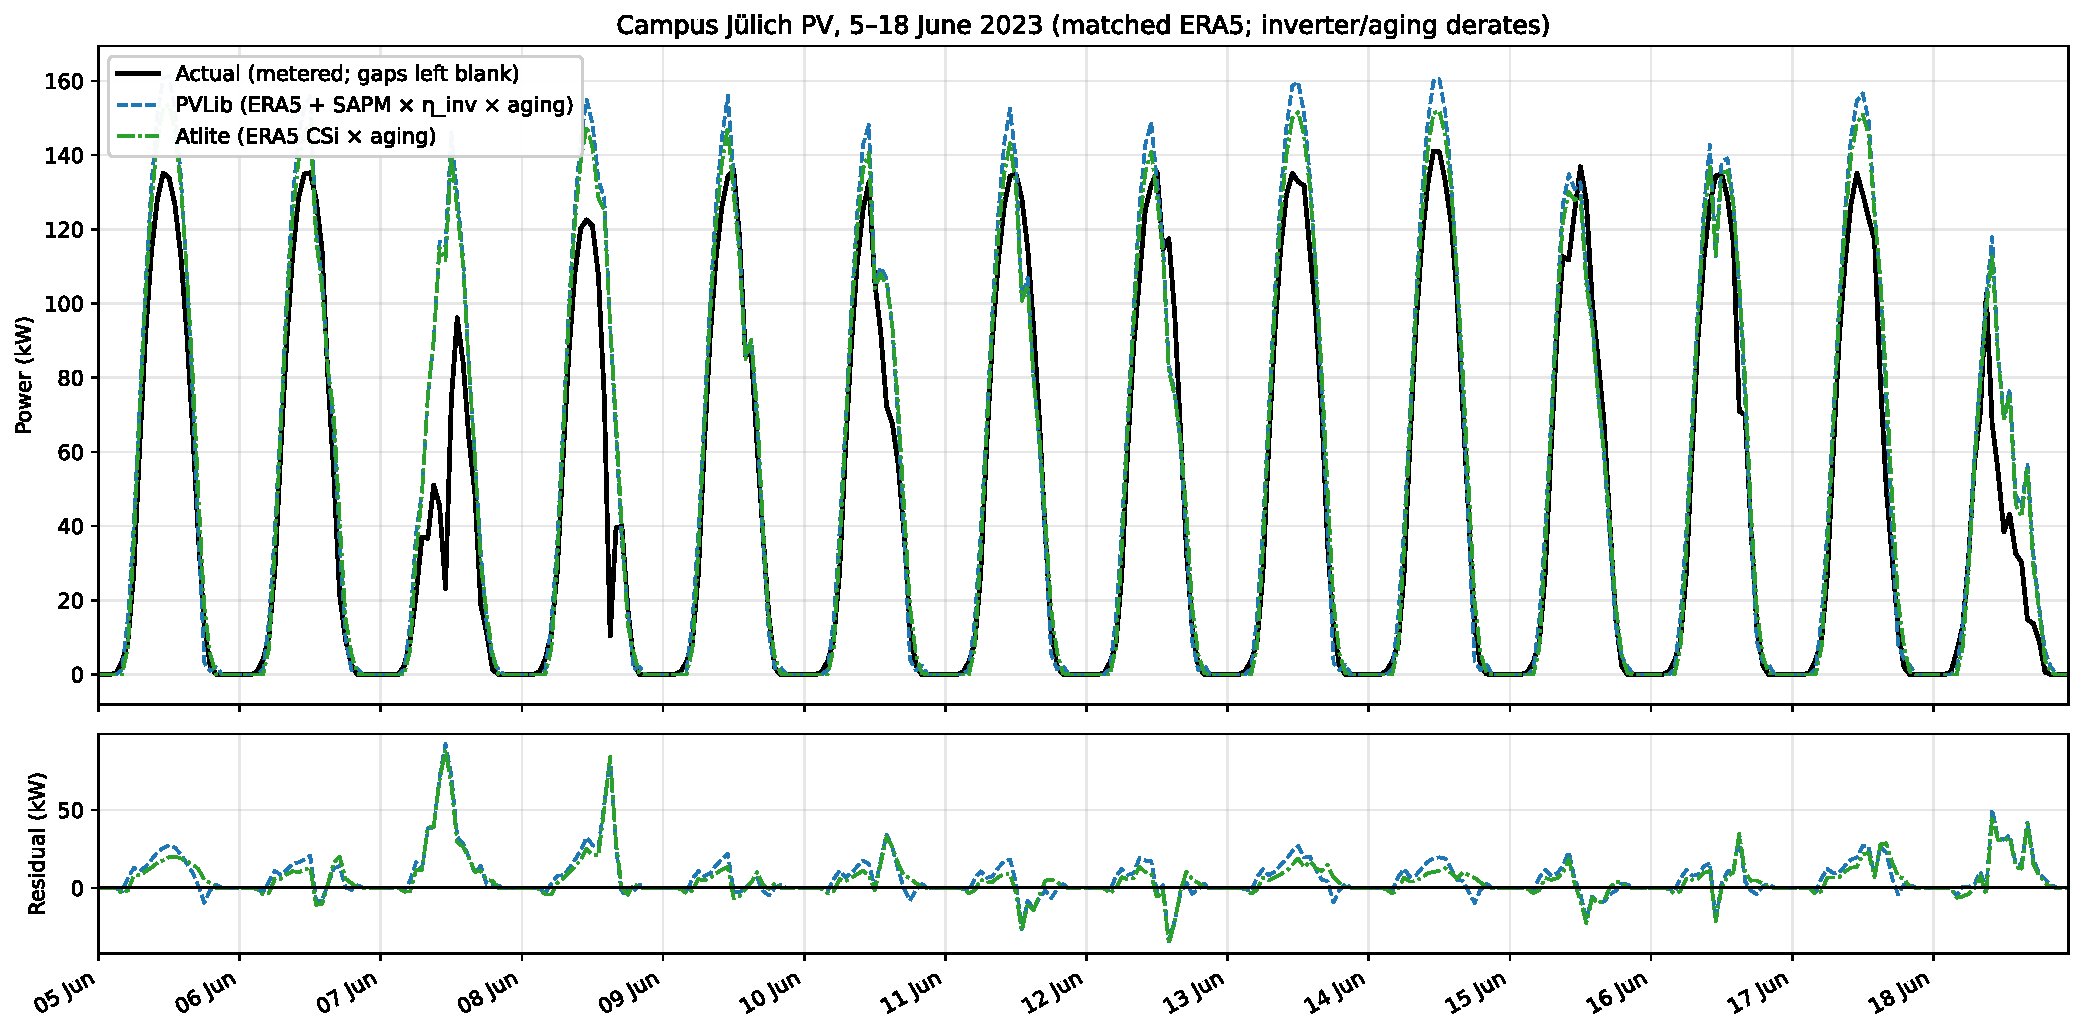
\includegraphics[width=14.0cm]{data/juelich_june_2weeks.pdf}
\caption{%
Campus Jülich PV, 5--18 June 2023: measured AC versus PVLib and Atlite on the same ERA5 cutout (inverter/aging derates).
Residual bias concentrates on clear peaks.\label{fig_juelich_june}
}

\end{figure}

\begin{figure}[htbp]
\centering
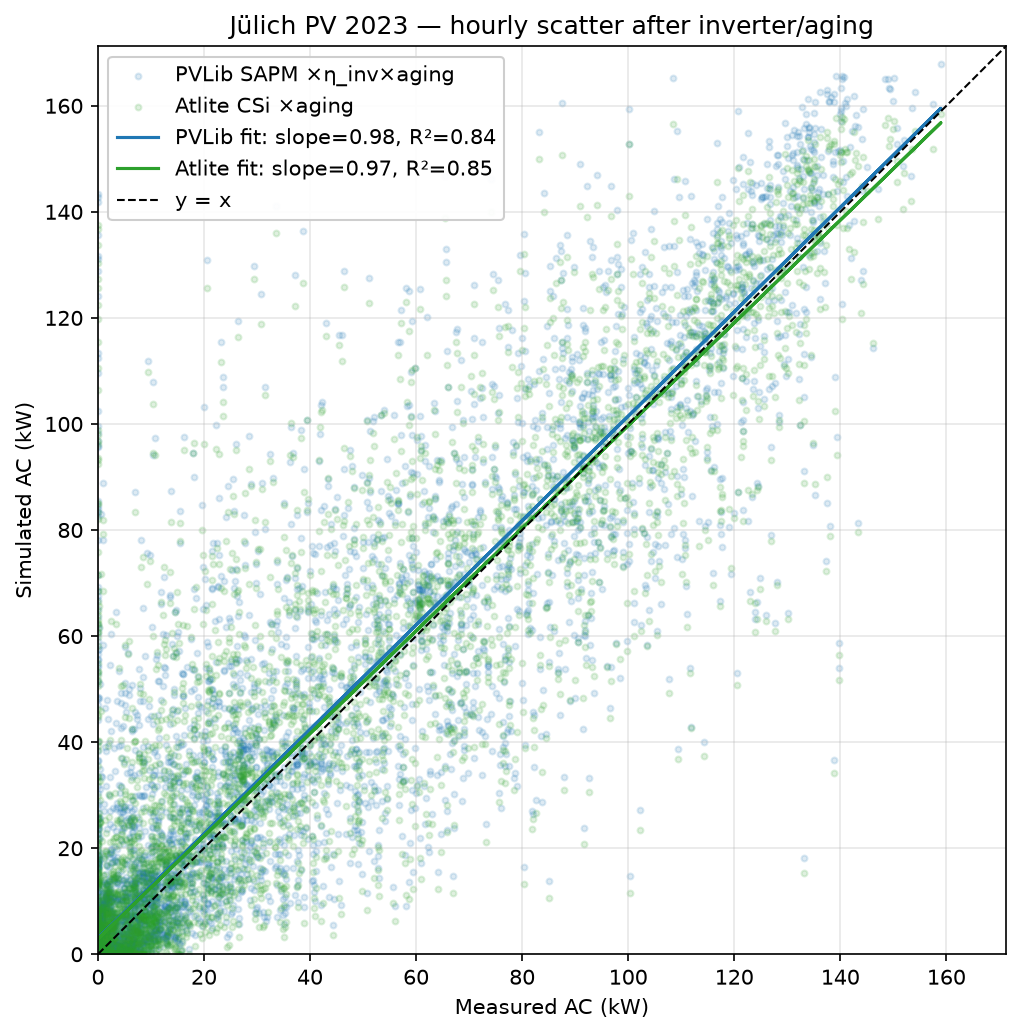
\includegraphics[width=11.0cm]{data/juelich_scatter_comparison.png}
\caption{%
Campus Jülich PV, 2023: hourly scatter of simulated versus measured AC after inverter/aging on the matched ERA5 cutout.
Libraries track the meter near $y=x$, with residual high-side bias on clear peaks.\label{fig_juelich_scatter}
}

\end{figure}

\begin{figure}[htbp]
\centering
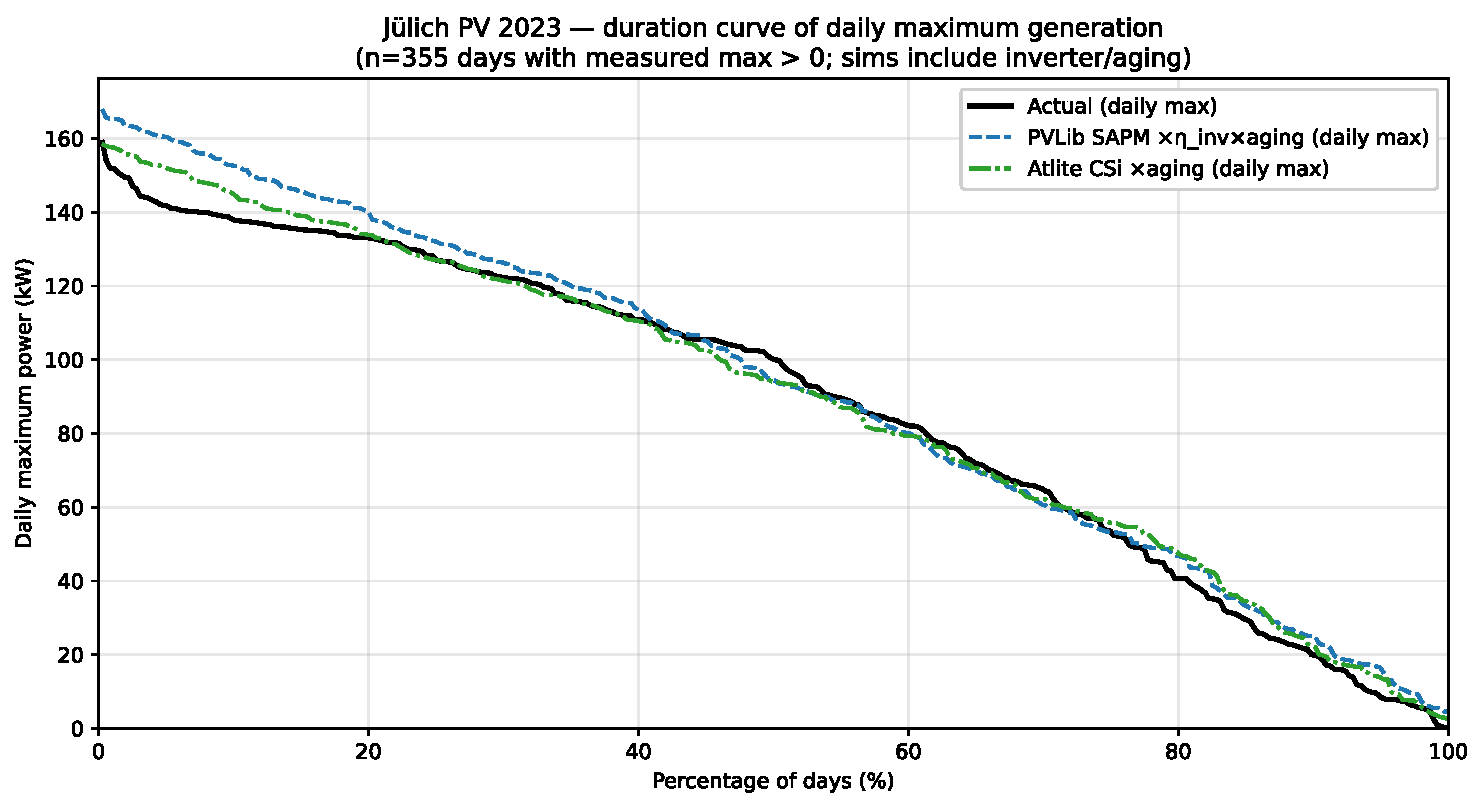
\includegraphics[width=12.0cm]{data/juelich_daily_max_duration.pdf}
\caption{%
Duration curve of daily maximum generation at Jülich, 2023.
The leftmost (highest) peaks---mostly clear summer days---remain the main residual overestimate after inverter and aging derates.\label{fig_juelich_dailymax_dur}
}

\end{figure}

Constant multipliers ($\eta_{\mathrm{inv}}$, aging) reduce energy bias and MAE/RMSE but cannot change Pearson $r$, which is scale-invariant.
SAPM trims the summer noon error by about $3$ percentage points in energy (Table~\ref{tab_juelich}), while the correlation improvement ($\Delta r \approx 0.001$) is negligible.
The practical lesson for modellers is that explicit, separately reported derates are more transparent than a single annual loss scalar---and for this plant, the $\sim$$10\%$ residual after derates sits squarely in the clear-sky tail where ERA5 irradiance is known to overshoot ground stations.

As a non-German library check, Kelmarsh wind farm SCADA (6$\times$2.05\,MW, UK) confirms that the two libraries sit within a few percentage points once both use ERA5 100\,m winds with the same shear model (Appendix~\ref{app:kelmarsh}).

%%%%%%%%%%%%%%%%%%%%%%%%%%%%%%%%%%%%%%%%%%
\section{TSO and National Seasonal Results}
\label{sec:national}

All national and TSO results use the shared ERA5 cutout.
Figure~\ref{fig_tso_map} shows the four German TSO zones and the Campus J{\"u}lich site for reference.
Figure~\ref{fig_seasonal_summary} and Table~\ref{tab_national_season} report national seasonal energy ratios and correlations versus ENTSO-E.
Figure~\ref{fig_tso_yield} (with Table~\ref{tab_tso_fy} for exact percentages) benchmarks the zones on the same cutout.
For wind, the national seasonal panel compares a MaStR-realistic Windpowerlib fleet with Atlite's single V112@80\,m setup---different fleets, not only different libraries.
For solar, both stacks are compared with ENTSO-E public-grid feed-in (Section~\ref{sec:solar_residual}).

\begin{figure}[htbp]
\centering
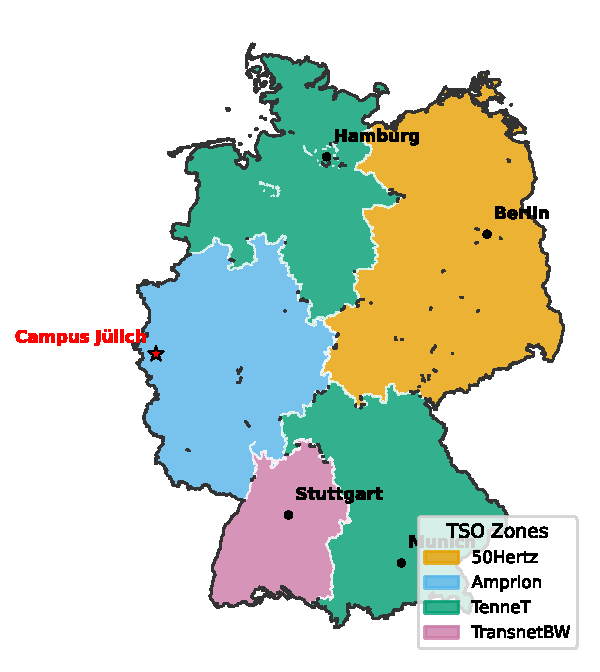
\includegraphics[width=8.0cm]{data/tso_zone_map.pdf}
\caption{%
The four German TSO zones (50Hertz, Amprion, TenneT, TransnetBW) and the Campus J{\"u}lich validation site ($\star$).
TenneT covers Schleswig-Holstein, much of Lower Saxony, and Bavaria; TransnetBW covers Baden-W{\"u}rttemberg.\label{fig_tso_map}
}

\end{figure}

\begin{figure}[htbp]
\centering
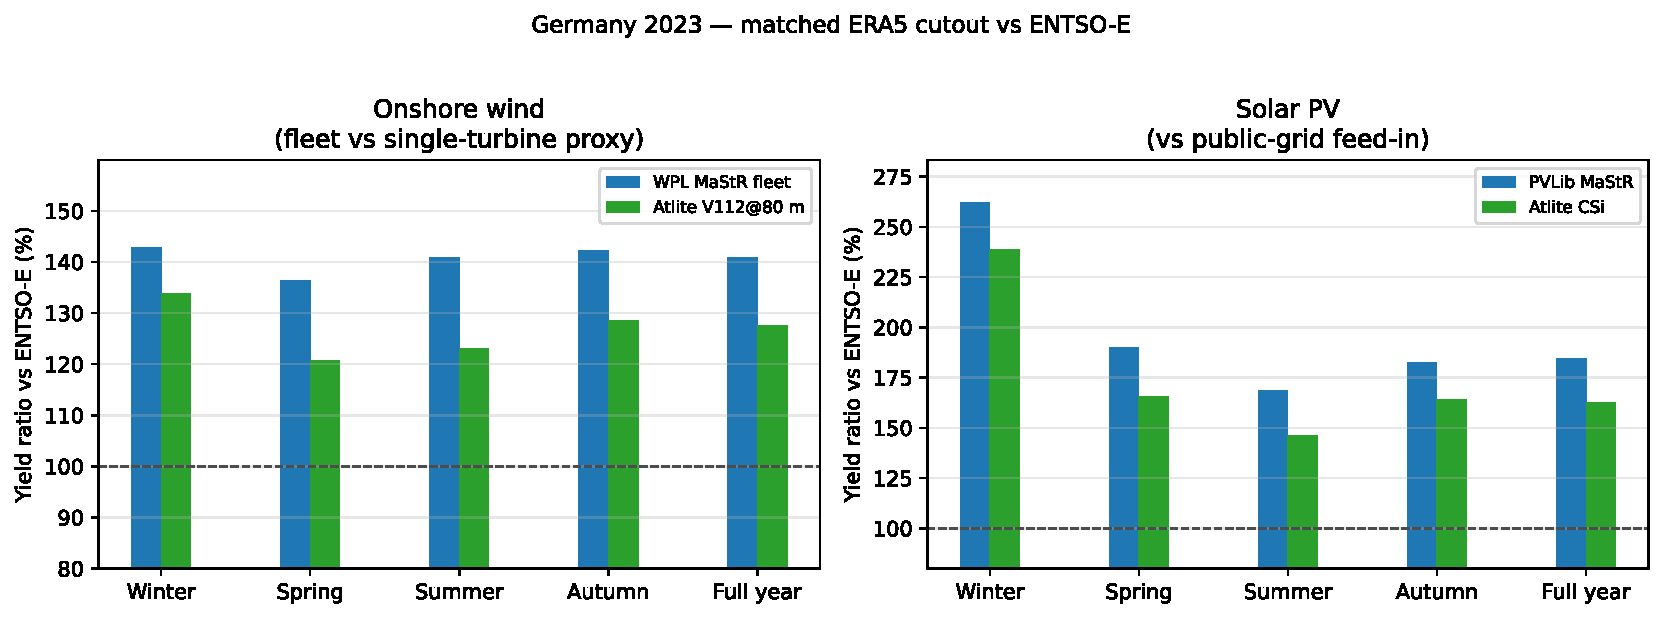
\includegraphics[width=14.0cm]{data/annual_seasonal_summary.pdf}
\caption{%
National seasonal yield ratios versus ENTSO-E, 2023, matched ERA5.
\emph{Left:} onshore wind---MaStR fleet (Windpowerlib) versus single-turbine V112@80\,m (Atlite).
\emph{Right:} solar PV versus public-grid feed-in.\label{fig_seasonal_summary}
}

\end{figure}

\begin{figure}[htbp]
\centering
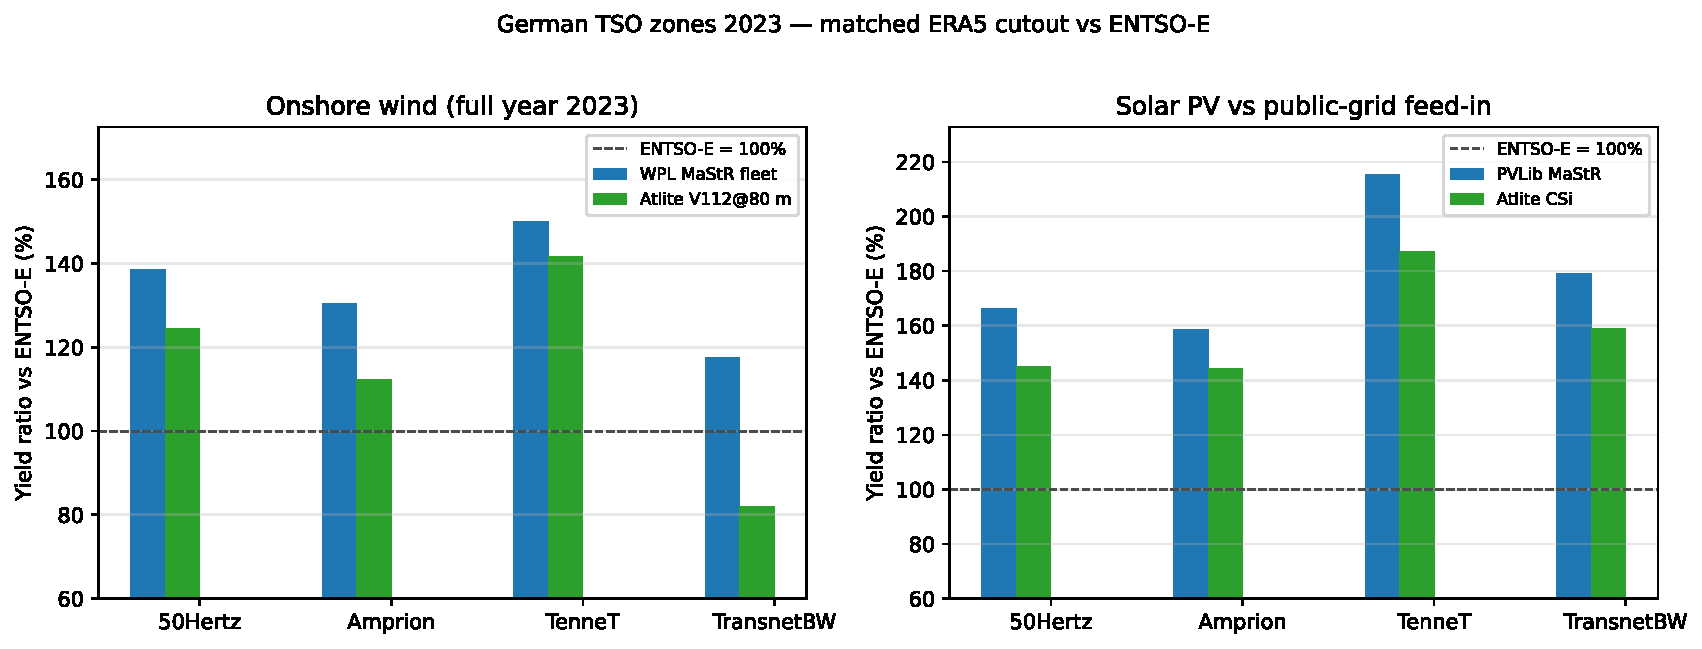
\includegraphics[width=14.0cm]{data/tso_yield_ratios.pdf}
\caption{%
Full-year 2023 TSO yield ratios versus ENTSO-E on the matched ERA5 cutout.
\emph{Left:} onshore wind---MaStR fleet (Windpowerlib) versus Atlite V112@80\,m.
\emph{Right:} solar PV versus public-grid feed-in (PVLib MaStR orientations).
Dashed line: ENTSO-E $=100\%$.
TransnetBW wind under Atlite ($82.1\%$) and TenneT solar (highest overshoot) are the clear spatial outliers.\label{fig_tso_yield}
}

\end{figure}

\begin{table}[htbp]
\caption{%
Germany national stacks versus ENTSO-E by season (matched ERA5).
Wind columns: Atlite V112@80\,m vs.\ Windpowerlib MaStR fleet (Section~\ref{sec:wind_fleet}).
Solar columns are raw (no national fleet aging); derated solar is in Table~\ref{tab_national_derates}.
Column keys: W = wind, S = solar, WPL = Windpowerlib, Atl.\ = Atlite; $r$ W and $r$ S are correlations of each stack versus ENTSO-E (WPL/Atlite for wind; PVLib/Atlite for solar).\label{tab_national_season}
}

\begin{tabularx}{\textwidth}{lcccccccc}
\toprule
\textbf{Season} & \textbf{W WPL} & \textbf{W Atl.} & \textbf{$r$ W} & \textbf{S PVLib} & \textbf{S Atl.} & \textbf{$r$ S}\\
\midrule
Winter & 143.0\% & 133.7\% & 0.963 / 0.962 & 262.2\% & 238.6\% & 0.838 / 0.896\\
Spring & 136.5\% & 120.7\% & 0.981 / 0.976 & 189.8\% & 165.6\% & 0.938 / 0.940\\
Summer & 140.9\% & 123.1\% & 0.968 / 0.961 & 168.6\% & 146.2\% & 0.957 / 0.951\\
Autumn & 142.4\% & 128.6\% & 0.988 / 0.984 & 182.5\% & 164.0\% & 0.911 / 0.932\\
Full year & 141.0\% & 127.7\% & 0.976 / 0.974 & 184.7\% & 162.5\% & 0.935 / 0.940\\
\bottomrule
\end{tabularx}
\end{table}

\begin{table}[htbp]
\caption{%
Full-year 2023 TSO yield ratios versus ENTSO-E (matched ERA5); companion numbers for Figure~\ref{fig_tso_yield}.
Wind: MaStR fleet vs.\ V112@80\,m (not fleet-matched).
Solar: raw vs.\ feed-in.\label{tab_tso_fy}
}

\begin{tabularx}{\textwidth}{lCCCC}
\toprule
\textbf{TSO} & \textbf{Wind WPL} & \textbf{Wind Atlite} & \textbf{Solar PVLib} & \textbf{Solar Atlite}\\
\midrule
50Hertz & 138.6\% & 124.5\% & 166.3\% & 145.2\%\\
Amprion & 130.7\% & 112.4\% & 158.6\% & 144.2\%\\
TenneT & 150.2\% & 141.8\% & 215.5\% & 187.0\%\\
TransnetBW & 117.7\% & 82.1\% & 179.1\% & 159.0\%\\
\bottomrule
\end{tabularx}
\end{table}

Both wind stacks track ENTSO-E chronologies (full-year $r\geq0.974$).
Under the default national setups the energy ratios are 127.7\% (Atlite V112@80\,m) and 141.0\% (Windpowerlib MaStR fleet).
That gap is mostly fleet representation (Section~\ref{sec:wind_fleet}).
TransnetBW is a spatial outlier for Atlite (82.1\% under-prediction amid national over-prediction); Windpowerlib is high but closer there (117.7\%).
Solar exceeds feed-in in every TSO; TenneT is highest (Section~\ref{sec:solar_residual}).
Figures~\ref{fig_tso_week_wind}--\ref{fig_tso_week_solar} show matched-ERA5 sample weeks for all four zones: chronologies track ENTSO-E, while energy bias remains.

\begin{figure}[htbp]
\centering
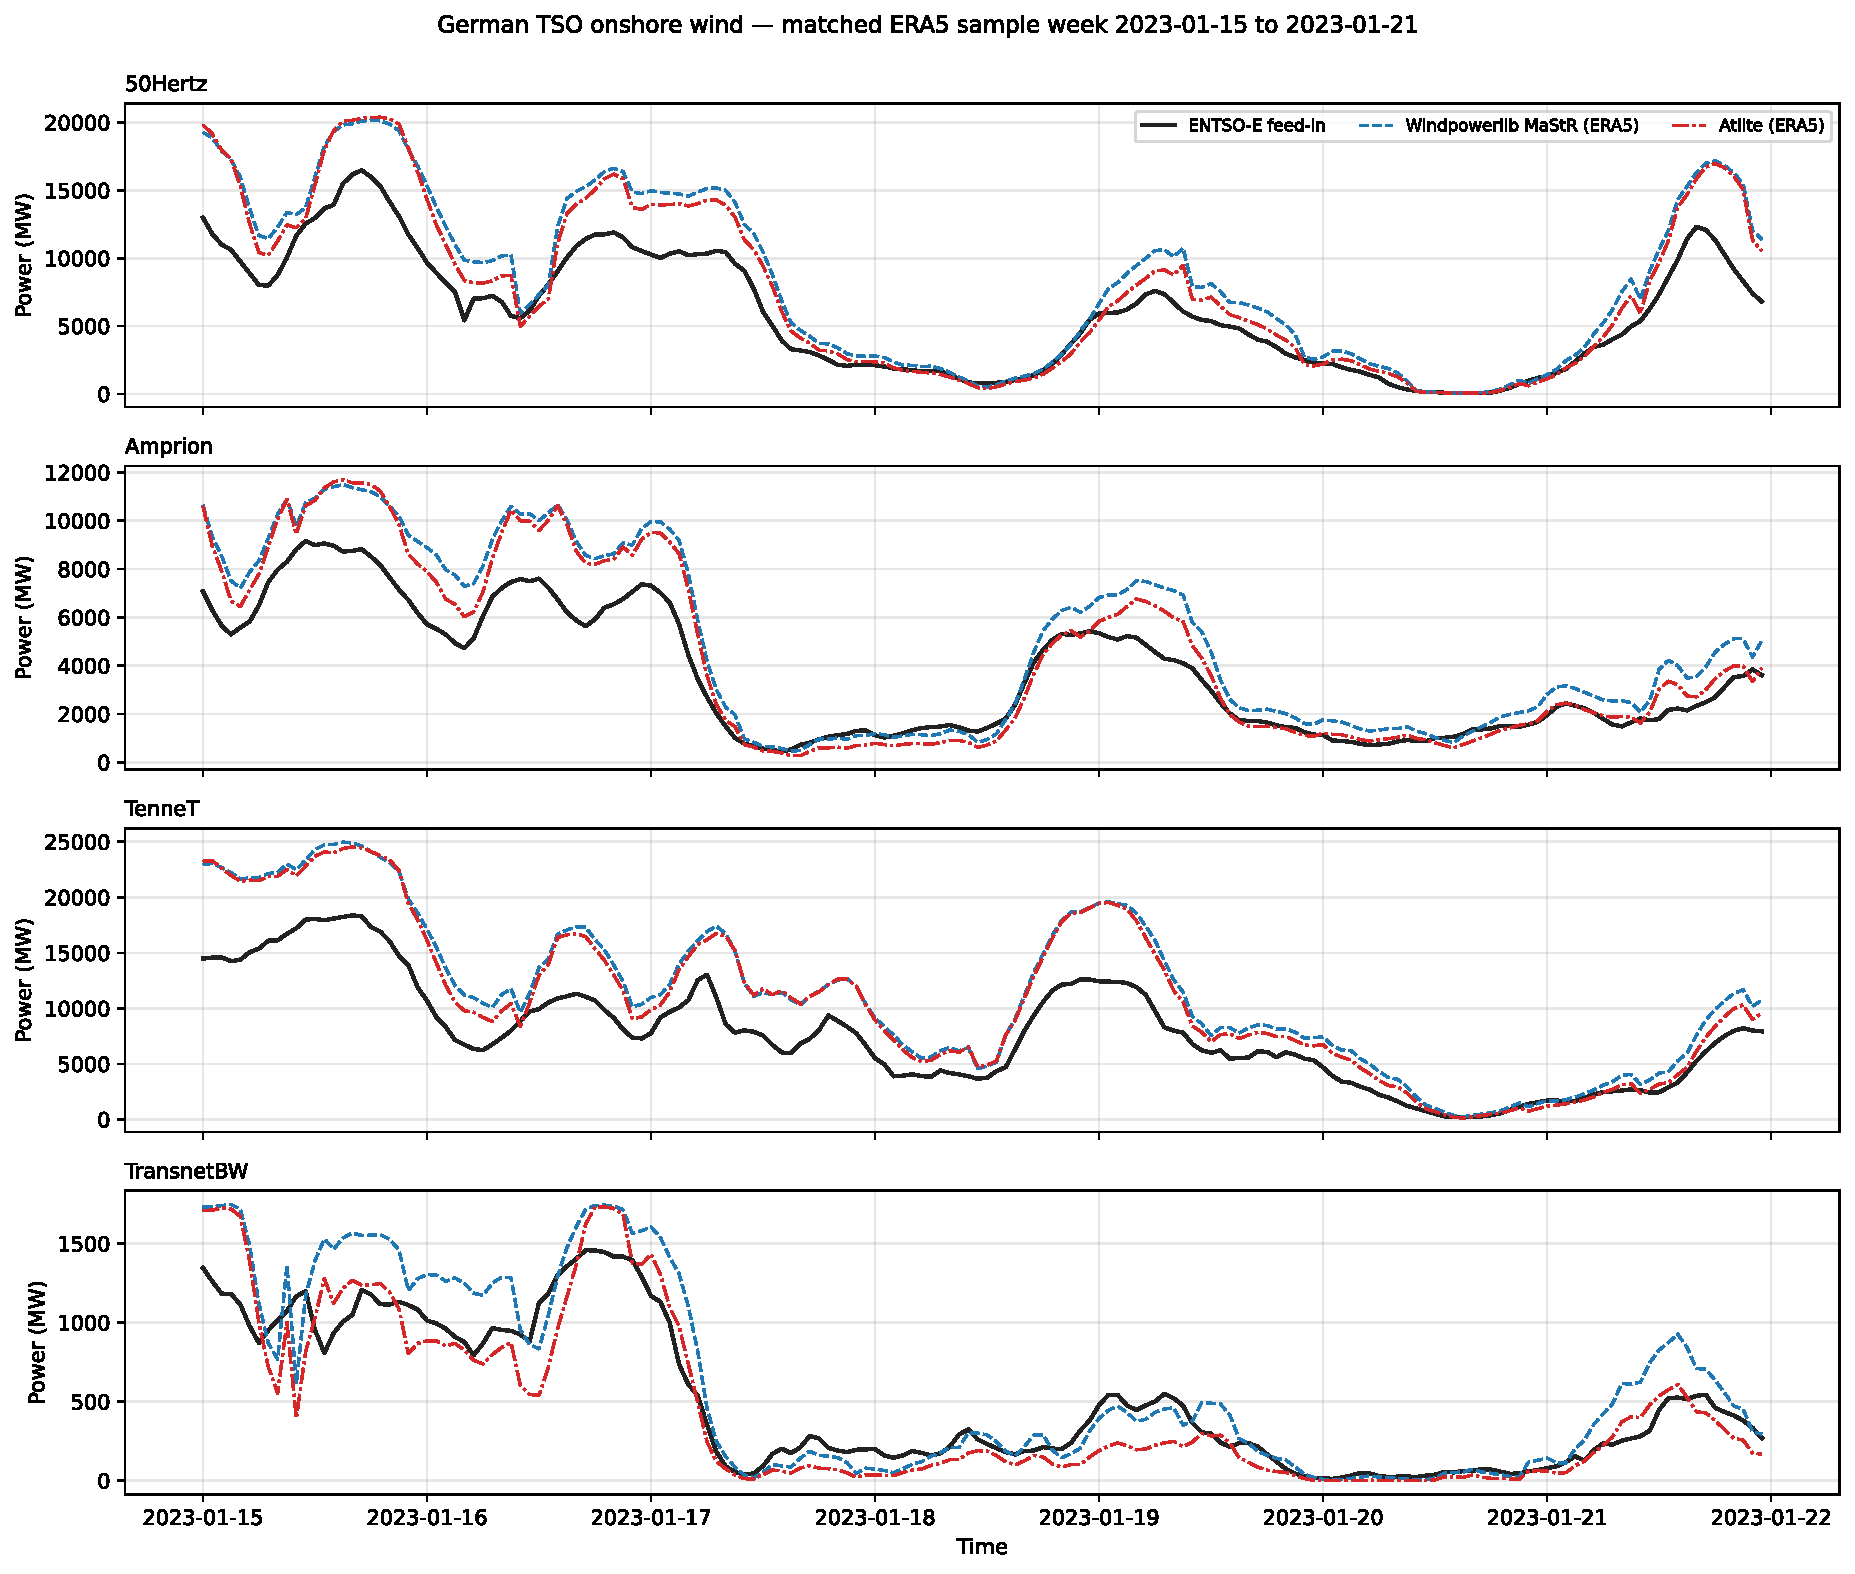
\includegraphics[width=14.0cm]{data/tso_matched_week_wind.pdf}
\caption{%
Matched ERA5 onshore-wind sample week (15--21 January 2023) for all four German TSO zones versus ENTSO-E feed-in.
Windpowerlib uses the MaStR fleet; Atlite uses V112@80\,m.\label{fig_tso_week_wind}
}

\end{figure}

\begin{figure}[htbp]
\centering
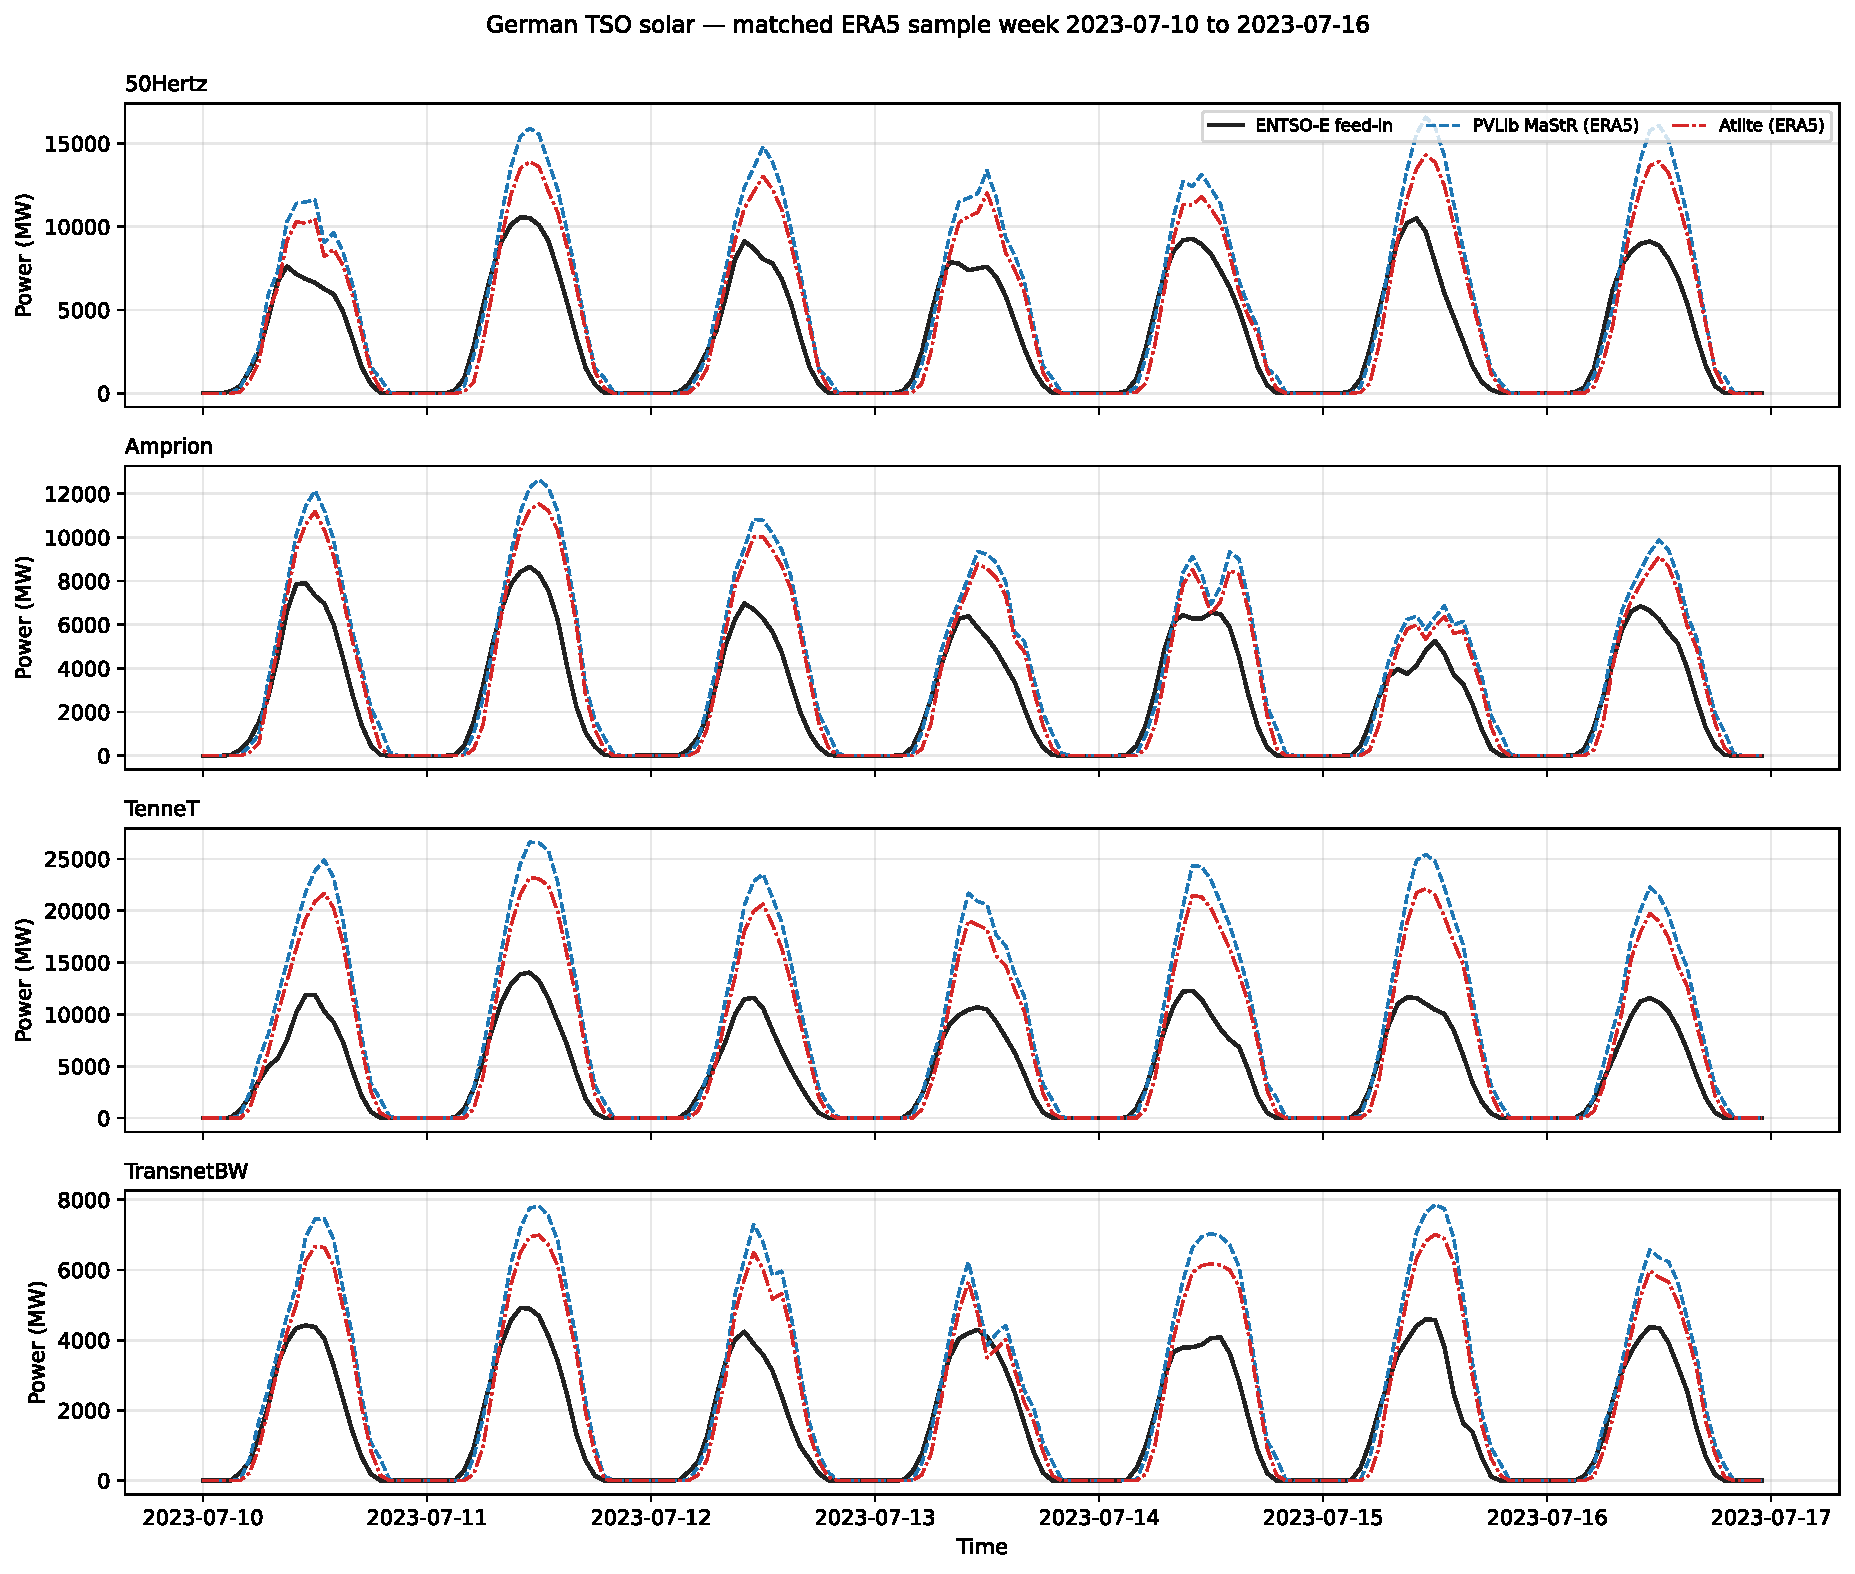
\includegraphics[width=14.0cm]{data/tso_matched_week_solar.pdf}
\caption{%
Matched ERA5 solar sample week (10--16 July 2023) for all four German TSO zones versus ENTSO-E public-grid feed-in.
Both stacks overshoot peaks systematically; TenneT shows the largest absolute gap.\label{fig_tso_week_solar}
}

\end{figure}

\subsection{Matched V112 library test versus MaStR fleet sensitivity}
\label{sec:wind_fleet}

To compare libraries fairly, turbine type and hub height are held fixed.
Forcing Windpowerlib onto Atlite's V112/3000 at 80\,m with Atlite-like log down-extrapolation from ERA5 100\,m yields 129.3\% of ENTSO-E versus Atlite's 127.7\% (Figure~\ref{fig_wind_library}; Table~\ref{tab_wind_v112}): Windpowerlib / Atlite $\sim$101\% ($r\approx1.00$).
The residual 1.6 pp between the matched libraries traces to differences in the oedb and Atlite power-curve tables at low-to-mid wind speeds.
Cut-out handling at 25\,m/s and the choice of NUTS3 centroid versus plant-level layout barely matter for a national annual total in Germany 2023.

The MaStR-fleet Windpowerlib run maps each unit to an oedb type by diameter and rated power and uses the reported hub (capacity-weighted mean $\sim$113\,m).
It yields 141.0\% of ENTSO-E and about $110\%$ of Atlite V112@80\,m.
We do not use coarse specific-power class aggregation for the national numbers.

\begin{figure}[htbp]
\centering
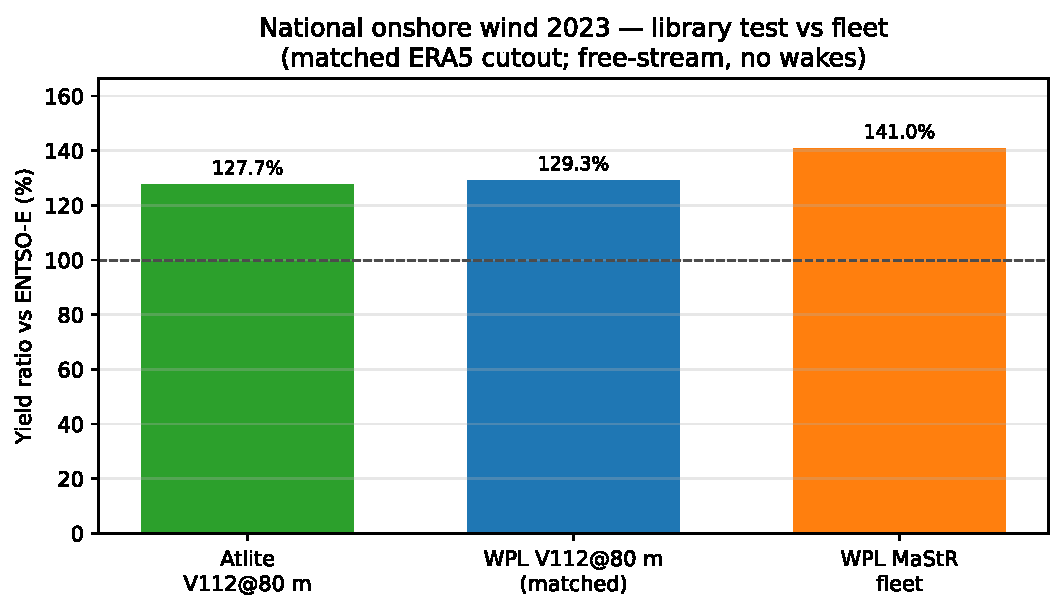
\includegraphics[width=10.0cm]{data/wind_library_test.pdf}
\caption{%
National onshore wind versus ENTSO-E, matched ERA5, 2023.
Matched V112@80\,m library test (left/centre) versus MaStR fleet sensitivity (right).
Fixing turbine and hub largely removes the library gap; the MaStR fleet remains higher as a free-stream multi-hub representation.\label{fig_wind_library}
}

\end{figure}

\begin{table}[htbp]
\caption{%
National onshore wind versus ENTSO-E, matched ERA5 cutout, 2023.
Matched V112@80\,m library test (top) and MaStR fleet sensitivity (bottom).\label{tab_wind_v112}
}

\begin{tabularx}{\textwidth}{lCCCC}
\toprule
\textbf{Configuration} & \textbf{Ratio (\%)} & \textbf{$r$} & \textbf{MAE (MW)} & \textbf{RMSE (MW)}\\
\midrule
Atlite V112 @ 80\,m & 127.7 & 0.974 & 4111 & 6538\\
Windpowerlib V112 @ 80\,m (matched proxy) & 129.3 & 0.974 & 4364 & 6980\\
Windpowerlib MaStR fleet (types + hubs) & 141.0 & 0.976 & 5612 & 7845\\
\bottomrule
\end{tabularx}
\end{table}

Neither stack applies park wakes, turbine availability, electrical losses, or grid curtailment: both convert free-stream hub wind through a power curve onto nameplate capacity.
Table~\ref{tab_wind_loss_budget} puts known terms next to the MaStR-fleet overshoot ($\sim$41\% vs.\ ENTSO-E).
Onshore Redispatch alone is $\sim$3.4\% of ENTSO-E onshore energy~\citep{SMARD2024Redispatch2023}---too small to close the gap.
Availability, electrical losses, ERA5 wind bias, and park wakes are not split out here; together they must account for most of the remaining overshoot.
The lower Atlite ratio (127.7\%) compared to the MaStR fleet (141.0\%) partly reflects Atlite's lower hub height (80\,m versus the MaStR capacity-weighted mean of $\sim$113\,m), but this offset is incidental---it does not substitute for an explicit wake or loss model.

\begin{table}[htbp]
\caption{%
Bounded national onshore-wind residual versus ENTSO-E (117.9\,TWh), MaStR-fleet free-stream run (141.0\%).
Known terms only; unknowns not ranked.\label{tab_wind_loss_budget}
}

\begin{tabularx}{\textwidth}{lCC}
\toprule
\textbf{Term} & \textbf{Approx.\ share of ENTSO-E} & \textbf{Status}\\
\midrule
MaStR-fleet free-stream overshoot & $\sim$41\% & Measured in this study\\
Onshore Redispatch 2023 & $\sim$3.4\% & Known~\citep{SMARD2024Redispatch2023}\\
Availability, electrical, wakes, ERA5 bias, other & residual & Not separately identified\\
\bottomrule
\end{tabularx}
\end{table}

\subsection{Solar residual versus ENTSO-E feed-in}
\label{sec:solar_residual}

ENTSO-E solar here is public-grid feed-in, not full generation~\citep{ENTSOEActualGeneration}.
Raw simulations still sit above feed-in in every season, including summer (146.2--168.6\% before fleet aging; Table~\ref{tab_national_season}), while $r$ versus feed-in stays around $0.94$.
Snow or soiling in winter alone cannot explain that pattern.

Table~\ref{tab_residual_budget} and Figure~\ref{fig_solar_budget} give a coarse annual energy budget after inverter/fleet-aging derates.
Literature BTM~\citep{FraunhoferISE2025SelfConsumption} closes about one-quarter of the feed-in gap; the leftover ($\sim$23--25\,TWh) is open.
National MaStR solar capacity is only $\sim$106--108\% of ENTSO-E nameplate, so inventory over-count is not enough.
TenneT is the clear energy outlier (raw $\sim$187--216\% of feed-in): MaStR/ENTSO-E capacity there is $\sim$117--121\% (end-2023 partly imputed), and capacity-normalized full-load-hour ratios stay $\sim$150--160\% in all TSO zones.
So TenneT combines a higher inventory ratio with the same structural feed-in gap.

\begin{figure}[htbp]
\centering
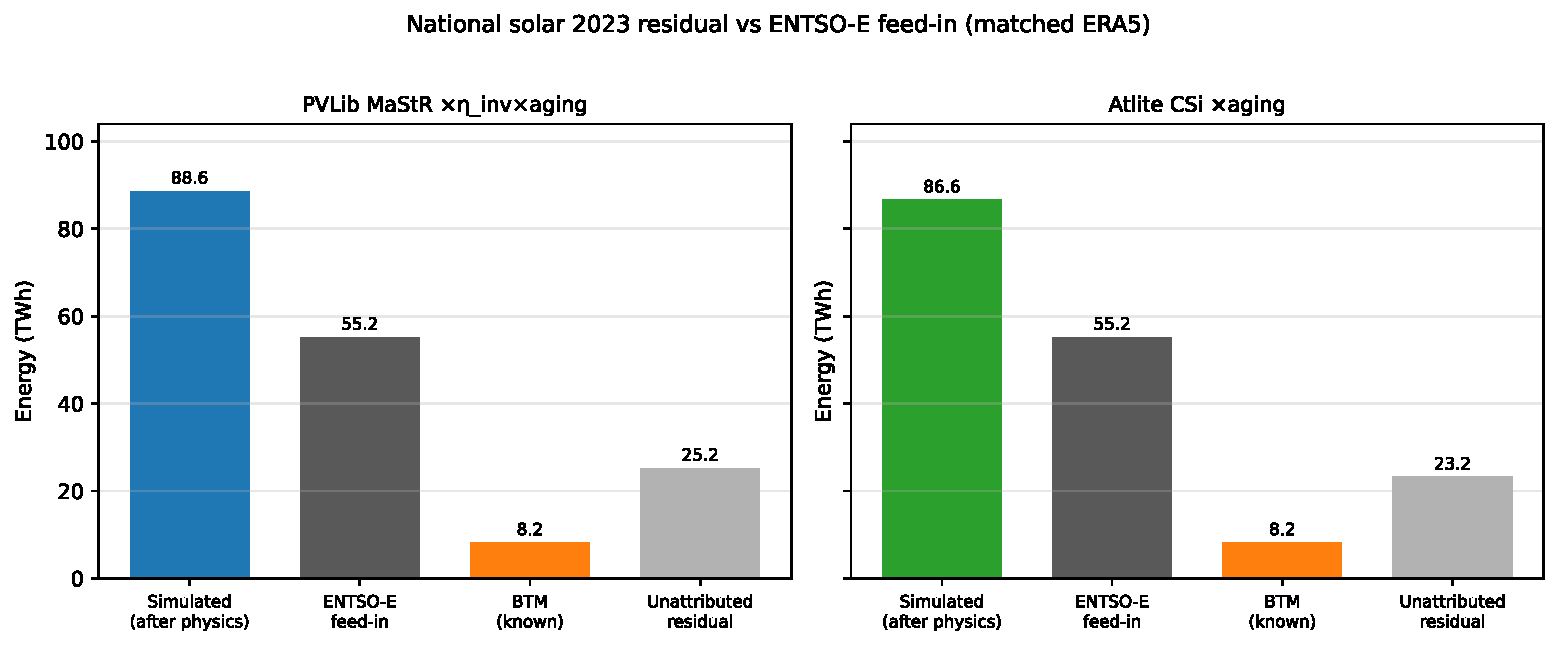
\includegraphics[width=12.5cm]{data/solar_residual_budget.pdf}
\caption{%
National solar energy residual for 2023 (TWh) after physics derates on the matched ERA5 cutout.
Bars: simulated generation, ENTSO-E public-grid feed-in, literature BTM ($8.2$\,TWh), and the unattributed remainder.\label{fig_solar_budget}
}

\end{figure}

\begin{table}[htbp]
\caption{%
National solar energy budget for 2023 (TWh), matched ERA5, versus ENTSO-E feed-in.
BTM $8.20$\,TWh from Fraunhofer ISE~\citep{FraunhoferISE2025SelfConsumption}.
Physics: PVLib $\eta_{\mathrm{inv}}\times\eta_{\mathrm{age}}$; Atlite $\eta_{\mathrm{age}}$ only.
National MaStR/ENTSO-E capacity ratio is $\sim$106--108\%.\label{tab_residual_budget}
}

\begin{tabularx}{\textwidth}{lCCl}
\toprule
\textbf{Quantity} & \textbf{PVLib (TWh)} & \textbf{Atlite (TWh)} & \textbf{Status}\\
\midrule
Simulated generation (after physics) & 88.6 & 86.6 & Computed\\
ENTSO-E solar feed-in & 55.2 & 55.2 & Measured\\
Gap to feed-in & 33.4 & 31.4 & \\
\midrule
Literature BTM self-consumption & 8.2 & 8.2 & Known~\citep{FraunhoferISE2025SelfConsumption}\\
Unattributed residual & 25.2 & 23.2 & Open\\
\bottomrule
\end{tabularx}
\end{table}

As a sanity check, we tried a constant energy-matching scalar ($\approx 0.62$) on top of the physics derates.
Annual sums match by construction, but the feed-in duration-curve shape does not recover (Appendix~\ref{app:national_derates}, Figure~\ref{fig_national_dailymax_dur}).
This confirms that the generation-to-feed-in gap is not a simple scale factor: behind-the-meter, curtailment, and estimation artefacts enter with their own temporal signatures.

\subsection{Wind: day versus night and TransnetBW}
\label{sec:wind_diurnal}

Day (06:00--17:00 UTC) and night (18:00--05:00 UTC) subsets on the matched ERA5 cutout (Table~\ref{tab_wind_daynight}) show roughly balanced overshoot nationally: the MaStR fleet sits at $\sim$140--142\% in both windows, and Atlite V112@80\,m at $\sim$126--129\%.
The same pattern holds at Kelmarsh once Windpowerlib also uses ERA5 100\,m + Hellman ($\sim$126--129\% day/night).
The absence of a diurnal bias structure confirms that the overshoot is a near-constant free-stream scaling issue on this cutout, not a stability- or shear-driven artefact.

TransnetBW stands out as an anomaly: Atlite V112@80\,m under-predicts there (82.1\% of ENTSO-E) while over-predicting nationally.
The most likely explanation is terrain: TransnetBW covers the Black Forest and the Swabian Alb, where ERA5's $\sim$30\,km grid cannot resolve orographic wind channelling, and where the V112 proxy may be poorly matched to the actual installed fleet.
Windpowerlib's MaStR fleet, which uses site-specific turbine types and hubs, is high there too (117.7\%) but much closer to ENTSO-E.

\begin{table}[htbp]
\caption{%
Wind day/night yield ratios and correlations, 2023.
Kelmarsh and national rows both use ERA5 100\,m winds (WPL: Hellman to hub; Atlite: log/roughness path).
Day = hours 06--17 UTC; night = 18--05 UTC.\label{tab_wind_daynight}
}

\begin{tabularx}{\textwidth}{lCCCCC}
\toprule
\textbf{Scale} & \textbf{Subset} & \textbf{WPL (\%)} & \textbf{Atlite (\%)} & \textbf{$r$ WPL} & \textbf{$r$ Atlite}\\
\midrule
Kelmarsh (farm) & Day & 125.9 & 126.6 & 0.907 & 0.905\\
Kelmarsh (farm) & Night & 129.0 & 135.1 & 0.902 & 0.899\\
Germany national & Day & 140.2 & 129.1 & 0.973 & 0.972\\
Germany national & Night & 141.5 & 126.3 & 0.980 & 0.976\\
\bottomrule
\end{tabularx}
\end{table}

%%%%%%%%%%%%%%%%%%%%%%%%%%%%%%%%%%%%%%%%%%
\section{Discussion}
\label{sec:discussion}

\subsection{Fleet matters more than the library}

The central result from the wind comparison is that a $14$ percentage-point gap between Windpowerlib and Atlite (141.0\% vs.\ 127.7\% of ENTSO-E) shrinks to about $2$ pp once both libraries use the same Vestas V112 at 80\,m.
For an energy-system modeller choosing between these stacks, the implication is direct: the turbine catalogue, the hub-height distribution, and the shear model will dominate national energy totals far more than any difference in the internal power-curve interpolation.
This is consistent with the farm-level result at Kelmarsh (Appendix~\ref{app:kelmarsh}), where both libraries sit within a few percentage points on the same SCADA benchmark.

The practical recommendation is therefore to fix the fleet first.
If two modelling teams use the same turbine and hub assumptions, their wind time series will agree at the $\sim$1--2\% level regardless of library---well within the noise introduced by ERA5 itself.
If they use different fleet representations, the library comparison is confounded and the resulting differences cannot be attributed.

\subsection{Solar: the benchmark problem}

On solar, the situation is more subtle.
At Campus J{\"u}lich---where we have measured AC from a known plant---the two stacks agree within $\sim$2\% of each other and sit about $10$--$12\%$ above the meter after inverter and aging derates.
That residual concentrates in clear-sky peaks and plausibly reflects ERA5 irradiance overshoot, not a library bug.

At national scale, the comparison shifts from a metering problem to a benchmarking problem.
ENTSO-E series report public-grid feed-in, not total generation: behind-the-meter self-consumption ($8.2$\,TWh, roughly $13\%$ of net generation) is absent from the reference.
After physics derates and literature BTM, a $\sim$23--25\,TWh gap remains (Table~\ref{tab_residual_budget}).
That gap is about $42$--$45\%$ of the reported feed-in and is dominated by the generation-to-feed-in boundary---curtailment, estimation methods in the Transparency Platform, timing of MaStR registrations, and possibly ERA5 irradiance bias---rather than by library deficiencies.

The seasonal colour decomposition in Figure~\ref{fig_national_scatter} shows that the overshoot is not concentrated in winter (where snow and low sun could explain it) but is spread across all seasons, consistent with a structural offset between simulated generation and reported feed-in.
TenneT's outsized ratio ($\sim$187--216\% of feed-in) coincides with the highest MaStR-to-ENTSO-E capacity ratio ($\sim$117--121\%), suggesting that inventory differences compound the feed-in gap there.

For modellers, the takeaway is that scoring raw simulated PV against ENTSO-E feed-in is a comparison of two different quantities.
Until a public German generation time series (including BTM) is available, the apparent overshoot should not be interpreted as a converter error alone.

\subsection{Limitations}
\label{sec:limitations}

This study covers one meteorological year (Germany 2023) on a single shared ERA5 cutout, with only one instrumented German PV plant.
The aging prior at J{\"u}lich is a documented estimate (mid-2011 commission, $\pm$2 years would shift the derate by $\pm$1 pp); the exact MaStR unit is not uniquely identified.
On wind, park wakes, turbine availability, electrical losses, and ERA5 wind bias are not separated; onshore Redispatch ($\sim$3.4\% of ENTSO-E wind energy~\citep{SMARD2024Redispatch2023}) is known but small.
The Kimber soiling check at J{\"u}lich uses a California rural prior on ERA5 precipitation and is not a calibrated national derate.
TransnetBW at $82.1\%$ under Atlite V112@80\,m is the spatial outlier (Figure~\ref{fig_tso_yield}); hub mix, roughness, and complex terrain in the Black Forest and the Swabian Alb are plausible explanations, but we did not isolate the cause.

%%%%%%%%%%%%%%%%%%%%%%%%%%%%%%%%%%%%%%%%%%
\section{Conclusions}
\label{sec:conclusions}

We compared Atlite and PVLib/Windpowerlib for Germany 2023 on a single ERA5 cutout, from a campus PV plant through four TSO zones to national ENTSO-E feed-in.
Two results stand out.
First, for national onshore wind, the apparent library gap is almost entirely a fleet gap: fixing the turbine and hub collapses a $14$ pp difference to $\sim$2 pp.
Second, for national solar, the dominant obstacle to validation is not the converter but the benchmark: ENTSO-E feed-in excludes behind-the-meter generation, and the $\sim$23--25\,TWh unattributed residual after BTM cannot be closed by physics derates alone.

For energy-system modellers, the practical advice is: calibrate your fleet assumptions before comparing libraries, and do not interpret a feed-in overshoot as a simulation error without accounting for the generation-to-feed-in boundary.
Future work should address park wakes and turbine availability on wind, and pursue generation-level solar benchmarks that include behind-the-meter production.

\section*{CRediT authorship contribution statement}
Conceptualization, F.M.; methodology, F.M.; software, F.M. and J.S.; validation, F.M. and J.S.; formal analysis, F.M. and J.S.; investigation, F.M. and J.S.; resources, V.S.; data curation, J.S.; writing---original draft preparation, F.M.; writing---review and editing, V.S., J.S. and J.R.; visualization, J.S.; supervision, V.S.
All authors have read and agreed to the published version of the manuscript.

\section*{Funding}
This research received no external funding.

\section*{Declaration of competing interest}
The authors declare that they have no known competing financial interests or personal relationships that could have appeared to influence the work reported in this paper.

\section*{Data availability}
Analysis code, pinned environment files, offline cache mode, timing logs, and aggregated comparison tables are available at \url{https://github.com/idt-fhac/atlite-pvlib-windpowerlib}.
Campus J{\"u}lich measured AC is publicly available via eview~\citep{eviewJuelich}; large ERA5 cutouts and Kelmarsh SCADA are available from the authors on reasonable request.

\appendix
\section{Campus Jülich PV: ablation, winter window, and hourly duration}
\label{app:juelich}

Table~\ref{tab_juelich_ablation} ablates temperature, inverter, and aging on meter-overlap hours.
Table~\ref{tab_juelich_windows} contrasts full-year metrics (8760\,h with meter gaps filled as zero) against overlap hours and daytime overlap.
Night and gap zeros shrink MAE/RMSE without improving daytime skill.
Figure~\ref{fig_juelich_jan} shows the January fortnight with snow from 19~January; Figure~\ref{fig_juelich_hourly_dur} is the hourly duration curve.
Main-text Figures~\ref{fig_juelich_june}, \ref{fig_juelich_scatter}, and \ref{fig_juelich_dailymax_dur} carry the June fortnight, scatter, and daily-maximum duration.

\paragraph{Kimber soiling sensitivity (site only).}
Applying \texttt{pvlib.soiling.kimber} on ERA5 total precipitation at the plant cell (rural loss rate $0.0011$\,d$^{-1}$, cleaning threshold $6$\,mm) shifts the PVLib overlap-hour ratio by about $-0.3$\,pp annually (largest seasonal hit $\sim$0.8\,pp in winter) with unchanged $r$.
This is a California rural prior on reanalysis rainfall---not a calibrated German derate---and does not close the $\sim$10\% meter gap.

\begin{table}[htbp]
\caption{%
Jülich factor ablation on meter-overlap hours (matched ERA5).
MAE/RMSE reductions are versus PVLib linear raw.
Constant factors do not raise correlation.\label{tab_juelich_ablation}
}

\begin{tabularx}{\textwidth}{lCCCC}
\toprule
\textbf{Configuration} & \textbf{Ratio (\%)} & \textbf{$r$} & \textbf{MAE $\downarrow$ (\%)} & \textbf{RMSE $\downarrow$ (\%)}\\
\midrule
PVLib linear (raw) & 132.6 & 0.8936 & 0.0 & 0.0\\
PVLib + SAPM (temp only) & 129.0 & 0.8941 & 8.5 & 9.9\\
PVLib linear $\times\eta_{\mathrm{inv}}$ & 119.4 & 0.8936 & 19.0 & 18.8\\
PVLib linear $\times$ aging & 124.7 & 0.8936 & 11.8 & 11.8\\
PVLib SAPM $\times\eta_{\mathrm{inv}}$ & 116.1 & 0.8941 & 26.1 & 25.9\\
PVLib SAPM $\times\eta_{\mathrm{inv}}\times$ aging & 109.2 & 0.8941 & 33.4 & 32.1\\
Atlite CSi (panel $\eta_{\mathrm{inv}}$) & 114.1 & 0.8993 & 30.8 & 29.9\\
Atlite $\times$ aging & 107.3 & 0.8993 & 37.5 & 35.3\\
\bottomrule
\end{tabularx}
\end{table}

\begin{table}[htbp]
\caption{%
Jülich absolute errors by time window after inverter/aging derates (matched ERA5).
Daytime = hours 07--17~UTC with measured power $>1$\,kW.\label{tab_juelich_windows}
}

\begin{tabularx}{\textwidth}{lCCCCC}
\toprule
\textbf{Model} & \textbf{Window} & \textbf{Ratio (\%)} & \textbf{$r$} & \textbf{MAE (kW)} & \textbf{RMSE (kW)}\\
\midrule
PVLib$\times\eta$ & Full year (gaps$\rightarrow$0) & 111.9 & 0.918 & 7.70 & 16.09\\
PVLib$\times\eta$ & Overlap hours & 109.2 & 0.894 & 13.80 & 20.47\\
PVLib$\times\eta$ & Daytime overlap & 108.9 & 0.865 & 16.50 & 22.86\\
Atlite$\times\eta_{\mathrm{age}}$ & Full year (gaps$\rightarrow$0) & 109.8 & 0.921 & 7.20 & 15.40\\
Atlite$\times\eta_{\mathrm{age}}$ & Overlap hours & 107.3 & 0.899 & 12.94 & 19.52\\
Atlite$\times\eta_{\mathrm{age}}$ & Daytime overlap & 107.3 & 0.871 & 15.45 & 21.79\\
\bottomrule
\end{tabularx}
\end{table}

\begin{figure}[htbp]
\centering
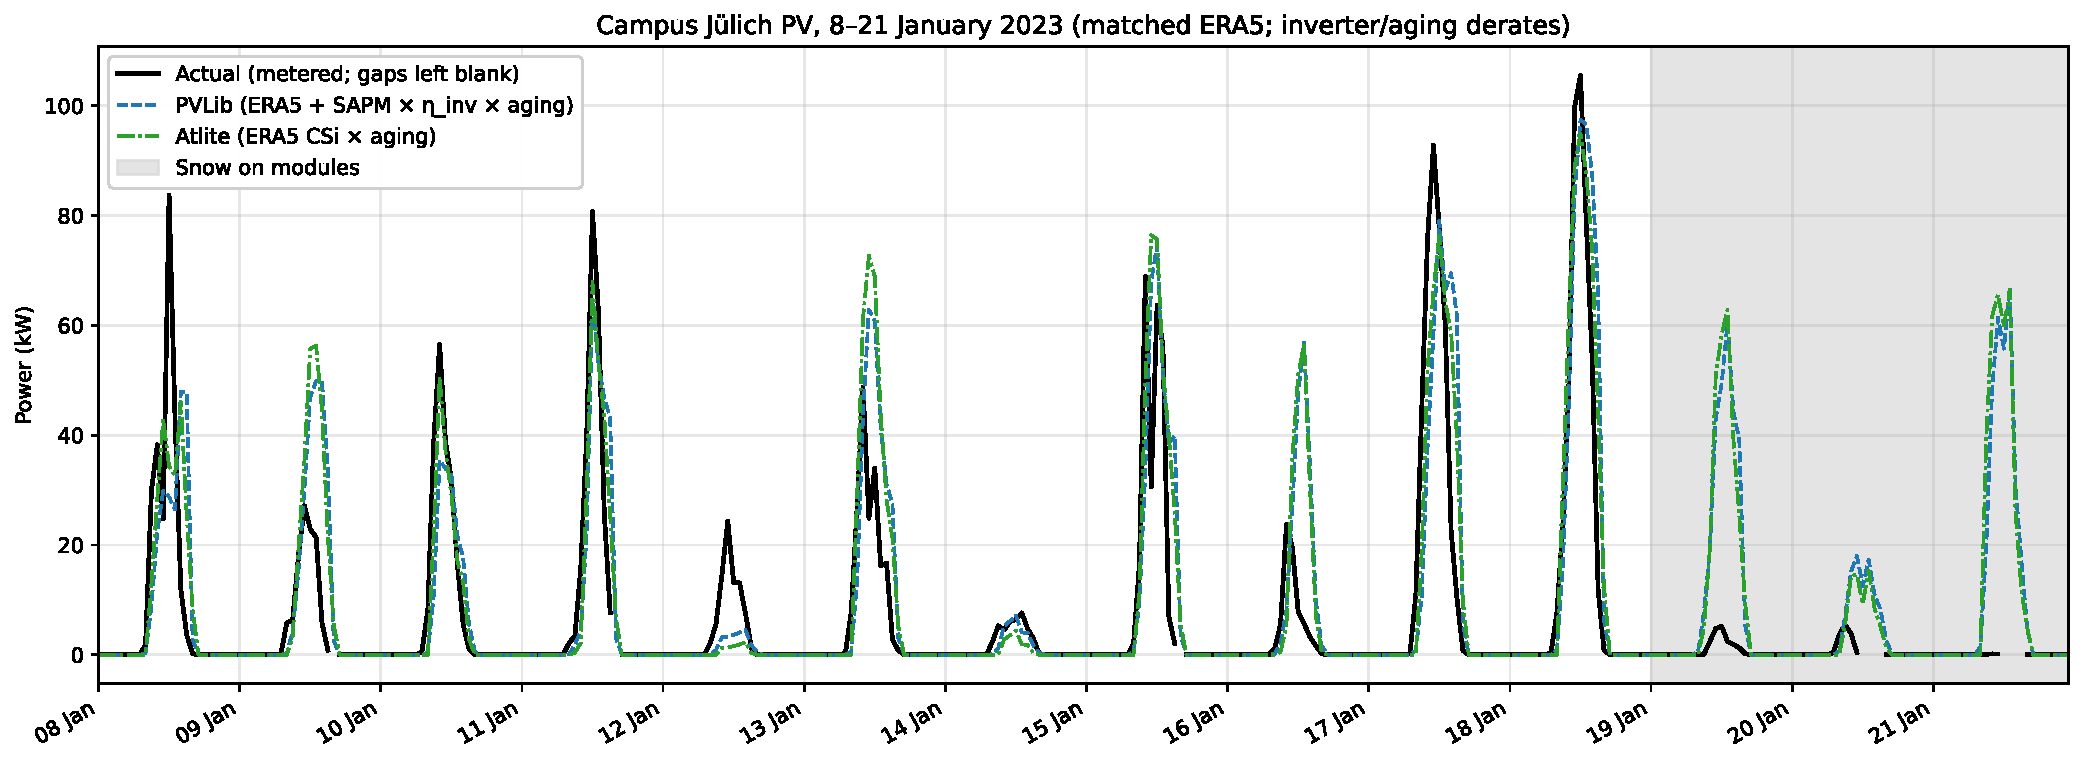
\includegraphics[width=14.0cm]{data/juelich_january_2weeks.pdf}
\caption{%
Campus Jülich PV, 8--21 January 2023: measured AC versus PVLib and Atlite on the same ERA5 cutout (inverter/aging derates).
Shaded: snow on modules from 19~January---an example of reality that free-stream conversion does not include.\label{fig_juelich_jan}
}

\end{figure}

\begin{figure}[htbp]
\centering
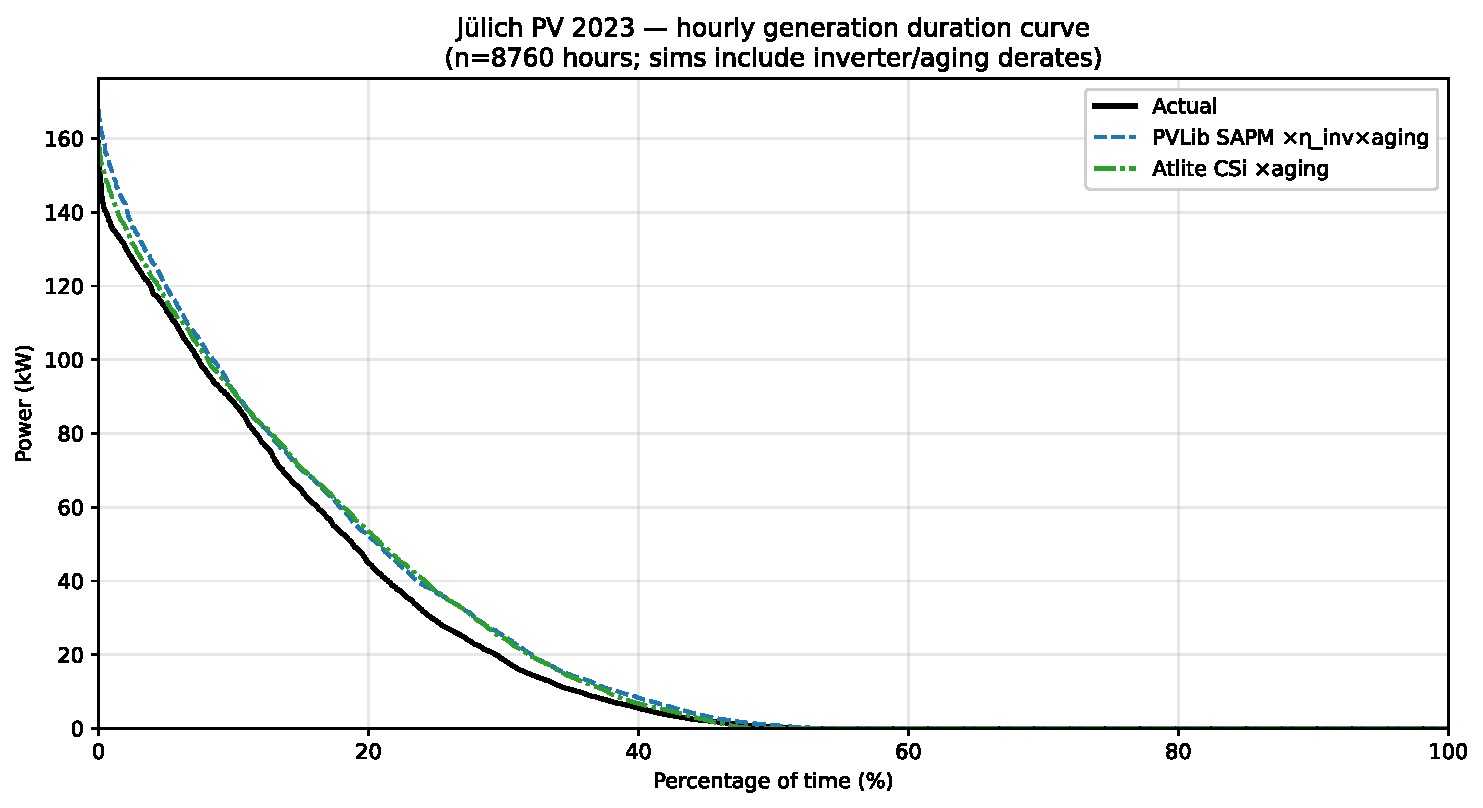
\includegraphics[width=12.0cm]{data/juelich_hourly_duration.pdf}
\caption{Hourly generation duration curve at Jülich, 2023 (overlap hours).\label{fig_juelich_hourly_dur}}
\end{figure}

\section{Kelmarsh wind farm (library check)}
\label{app:kelmarsh}

Kelmarsh (6$\times$Senvion MM92, 2.05\,MW each) is a UK wind farm with public SCADA data.
On the same ERA5 100\,m fields used nationally (Hellman shear to each turbine hub), Windpowerlib yields 127.4\% of farm SCADA (corr.\ 0.905); Atlite 130.8\% (0.902).
Day/night splits stay roughly balanced for both (Table~\ref{tab_wind_daynight}).
We use Kelmarsh only as a non-German library sanity check---not to calibrate German surface roughness or to draw national conclusions.
The result is consistent with the national matched-V112 test: once both libraries use the same turbine and hub, they agree to within a few percentage points.

\section{National matched-ERA5 solar with inverter and fleet aging}
\label{app:national_derates}

Applying the same physics stack nationally on the matched ERA5 cutout---PVLib $\eta_{\mathrm{inv}}=0.90$, capacity-weighted MaStR fleet aging $\eta_{\mathrm{age}}=0.966$ (mean age $6.9$\,y at $0.5\,\%$/y), Atlite aging only---reduces full-year yield versus ENTSO-E feed-in from $184.7\%$ to $160.6\%$ (PVLib MaStR) and from $162.5\%$ to $156.9\%$ (Atlite) (Table~\ref{tab_national_derates}).
Correlations are unchanged.
Versus feed-in plus literature BTM ($8.2$\,TWh), ratios remain $\sim$137--140\%.
Unlike Jülich measured AC ($\sim$110\% after derates), the national leftover is dominated by scoring against feed-in rather than generation---not by omitting inverter or aging alone.

Figure~\ref{fig_national_dailymax_dur} shows the duration curve of daily maxima for physics-derated generation versus ENTSO-E feed-in.
Figures~\ref{fig_national_scatter}--\ref{fig_national_scatter_scaled} show the corresponding hourly scatters without and with a trial constant scalar ($\approx 0.62$).
Energy matching lines up annual sums, but the cloud does not collapse onto $y=x$: behind-the-meter generation, curtailment, and estimation artefacts introduce temporal structure that a flat scalar cannot reproduce (Section~\ref{sec:solar_residual}).

\begin{table}[htbp]
\caption{Germany national solar versus ENTSO-E feed-in, matched ERA5 cutout, with and without inverter/fleet-aging derates (2023).\label{tab_national_derates}}
\begin{tabularx}{\textwidth}{lCCCC}
\toprule
\textbf{Configuration} & \textbf{Ratio (\%)} & \textbf{$r$} & \textbf{MAE (MW)} & \textbf{RMSE (MW)}\\
\midrule
PVLib MaStR raw & 184.7 & 0.935 & 5679 & 10087\\
PVLib MaStR $\times\eta_{\mathrm{inv}}\times\eta_{\mathrm{age}}$ & 160.6 & 0.935 & 4302 & 7616\\
Atlite CSi raw & 162.5 & 0.940 & 4557 & 7987\\
Atlite $\times\eta_{\mathrm{age}}$ & 156.9 & 0.940 & 4245 & 7418\\
\bottomrule
\end{tabularx}
\end{table}

\begin{figure}[htbp]
\centering
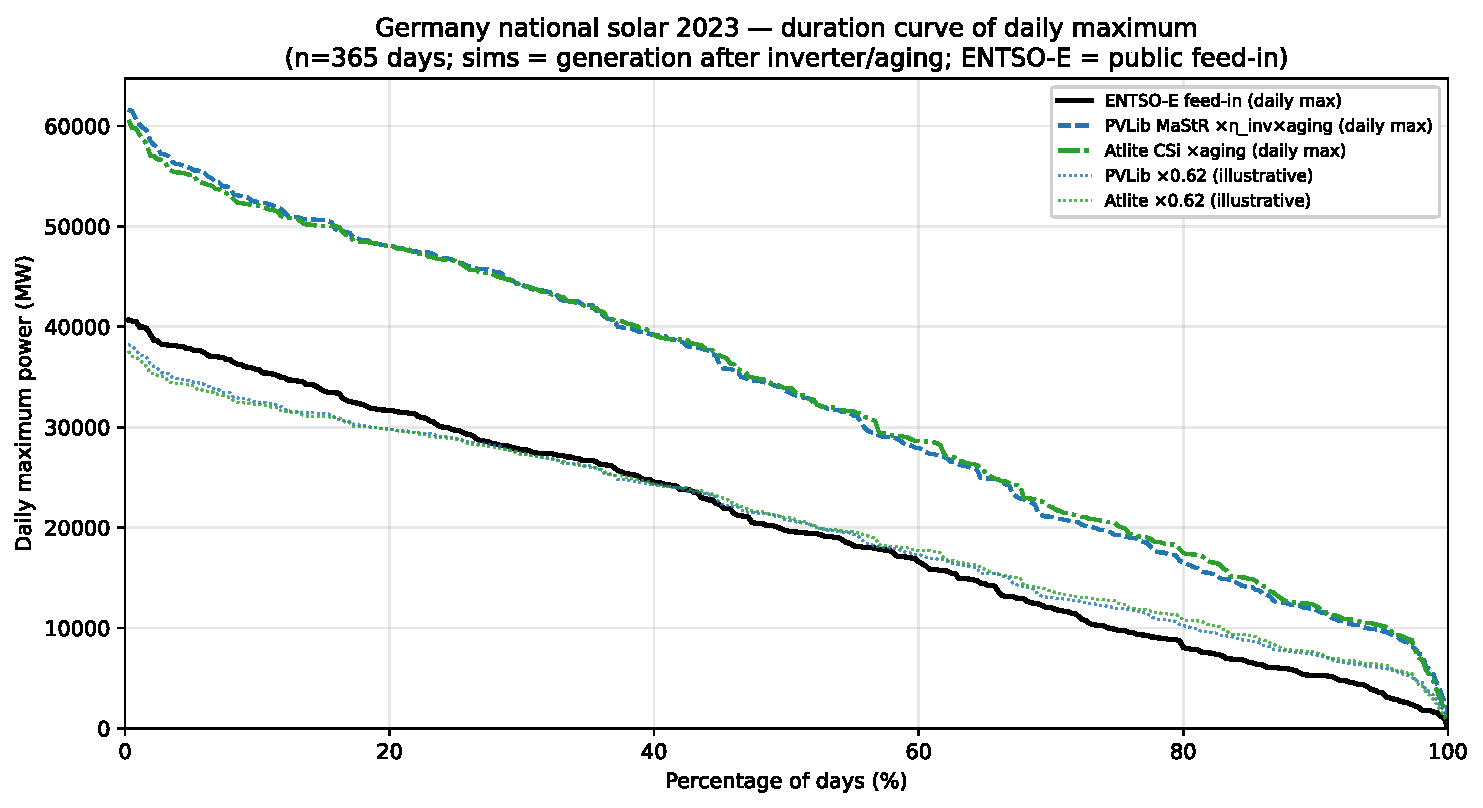
\includegraphics[width=12.0cm]{data/national_daily_max_duration.pdf}
\caption{%
Germany national solar 2023: duration curve of daily maximum power.
Simulated generation after inverter/fleet-aging (dotted) versus ENTSO-E public-grid feed-in (solid)~\citep{ENTSOEActualGeneration}.
Dashed curves show an illustrative energy-matching scalar ($\times 0.62$); annual sums align, but the feed-in characteristic is not recovered---the residual is left for future work.\label{fig_national_dailymax_dur}
}

\end{figure}

\begin{figure}[htbp]
\centering
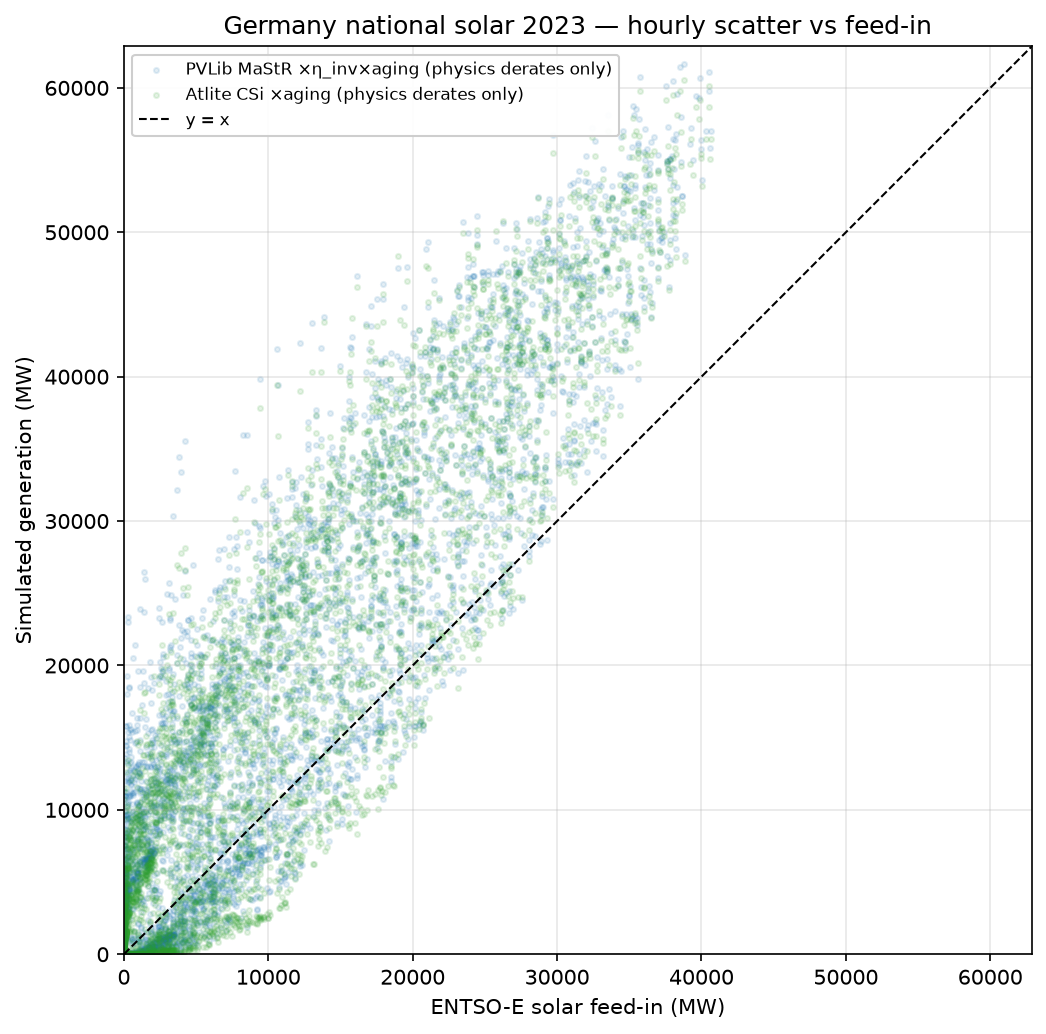
\includegraphics[width=11.0cm]{data/national_solar_scatter.png}
\caption{%
Germany national solar 2023: hourly scatter of physics-derated generation (PVLib $\times\eta_{\mathrm{inv}}\times\eta_{\mathrm{age}}$, Atlite $\times\eta_{\mathrm{age}}$) versus ENTSO-E public-grid feed-in~\citep{ENTSOEActualGeneration}.
The cloud lies systematically above $y=x$.\label{fig_national_scatter}
}

\end{figure}

\begin{figure}[htbp]
\centering
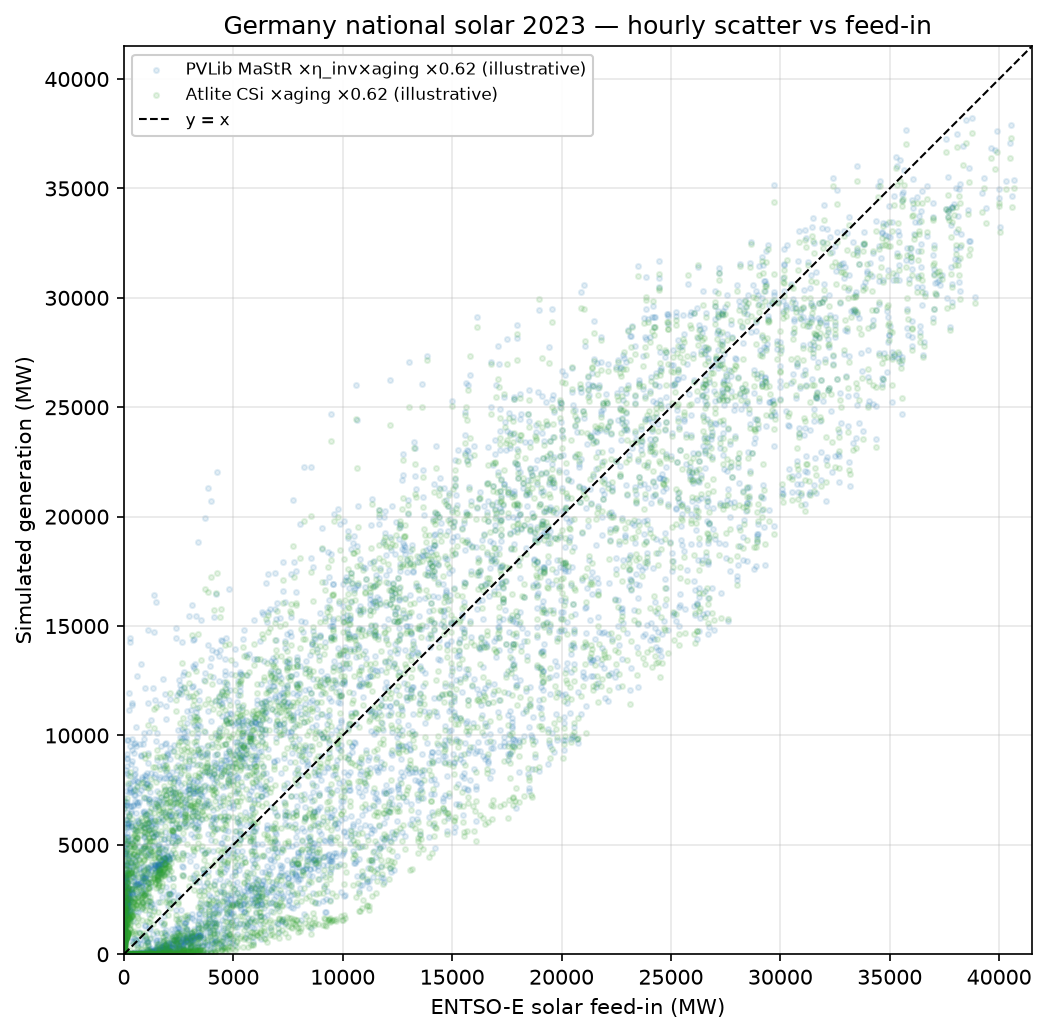
\includegraphics[width=11.0cm]{data/national_solar_scatter_scaled.png}
\caption{%
Same as Figure~\ref{fig_national_scatter}, after an illustrative constant energy-matching scalar ($\times 0.62$).
Annual energy is matched by construction, but the hourly cloud does not collapse onto $y=x$---the residual is left for future work.\label{fig_national_scatter_scaled}
}

\end{figure}

\bibliographystyle{elsarticle-num}
\bibliography{references}

\end{document}
